% NOTE: A25 is missing costars and subvars plot -- CHECK ASAP 


\documentclass{article}\usepackage[]{graphicx}\usepackage[]{color}

\usepackage[margin=0.35in]{geometry}
\usepackage{verbatim}
\usepackage{graphicx}
\usepackage{sidecap}
\usepackage{wrapfig}
\usepackage{textpos}



\makeatletter
\def\maxwidth{ %
  \ifdim\Gin@nat@width>\linewidth
    \linewidth
  \else
    \Gin@nat@width
  \fi
}
\makeatother

\definecolor{fgcolor}{rgb}{0.345, 0.345, 0.345}
\newcommand{\hlnum}[1]{\textcolor[rgb]{0.686,0.059,0.569}{#1}}%
\newcommand{\hlstr}[1]{\textcolor[rgb]{0.192,0.494,0.8}{#1}}%
\newcommand{\hlcom}[1]{\textcolor[rgb]{0.678,0.584,0.686}{\textit{#1}}}%
\newcommand{\hlopt}[1]{\textcolor[rgb]{0,0,0}{#1}}%
\newcommand{\hlstd}[1]{\textcolor[rgb]{0.345,0.345,0.345}{#1}}%
\newcommand{\hlkwa}[1]{\textcolor[rgb]{0.161,0.373,0.58}{\textbf{#1}}}%
\newcommand{\hlkwb}[1]{\textcolor[rgb]{0.69,0.353,0.396}{#1}}%
\newcommand{\hlkwc}[1]{\textcolor[rgb]{0.333,0.667,0.333}{#1}}%
\newcommand{\hlkwd}[1]{\textcolor[rgb]{0.737,0.353,0.396}{\textbf{#1}}}%

\usepackage{framed}
\makeatletter
\newenvironment{kframe}{%
 \def\at@end@of@kframe{}%
 \ifinner\ifhmode%
  \def\at@end@of@kframe{\end{minipage}}%
  \begin{minipage}{\columnwidth}%
 \fi\fi%
 \def\FrameCommand##1{\hskip\@totalleftmargin \hskip-\fboxsep
 \colorbox{shadecolor}{##1}\hskip-\fboxsep
     % There is no \\@totalrightmargin, so:
     \hskip-\linewidth \hskip-\@totalleftmargin \hskip\columnwidth}%
 \MakeFramed {\advance\hsize-\width
   \@totalleftmargin\z@ \linewidth\hsize
   \@setminipage}}%
 {\par\unskip\endMakeFramed%
 \at@end@of@kframe}
\makeatother

\definecolor{shadecolor}{rgb}{.97, .97, .97}
\definecolor{messagecolor}{rgb}{0, 0, 0}
\definecolor{warningcolor}{rgb}{1, 0, 1}
\definecolor{errorcolor}{rgb}{1, 0, 0}
\newenvironment{knitrout}{}{} % an empty environment to be redefined in TeX

\usepackage{alltt}
\usepackage{amsmath}
\usepackage{amssymb}
\usepackage{graphicx}
\IfFileExists{upquote.sty}{\usepackage{upquote}}{}
\begin{document}

\begin{knitrout}
\definecolor{shadecolor}{rgb}{0.969, 0.969, 0.969}\color{fgcolor}
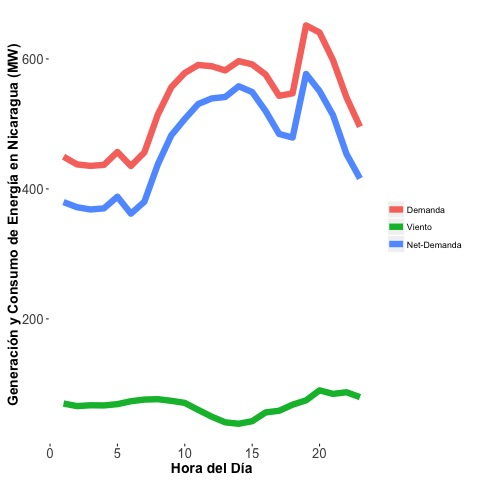
\includegraphics[scale=0.65]{figure/gridplot1.jpg} 
\end{knitrout}

 \begin{textblock}{1}(9,-5)
\begin{minipage}{20em}
\begingroup
\input{grid_text1.txt}
\endgroup
\end{minipage}
\end{textblock}

 \vspace{2cm}

\begin{knitrout}
\definecolor{shadecolor}{rgb}{0.969, 0.969, 0.969}\color{fgcolor}
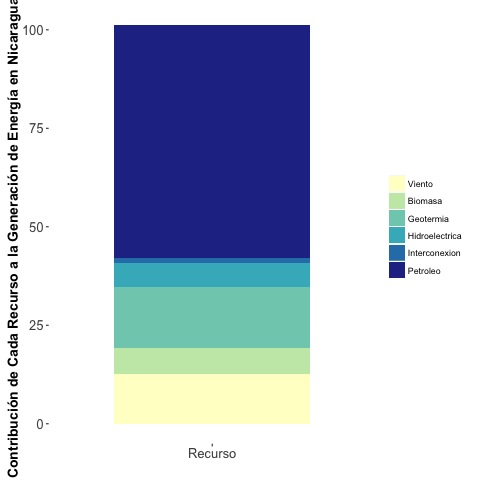
\includegraphics[scale=0.65]{figure/gridplot2.jpg} 
\end{knitrout}

 \begin{textblock}{1}(9,-5)
\begin{minipage}{20em}
\begingroup
\input{grid_text2.txt}
\endgroup
\end{minipage}
\end{textblock}

\begin{knitrout}
\definecolor{shadecolor}{rgb}{0.969, 0.969, 0.969}\color{fgcolor}
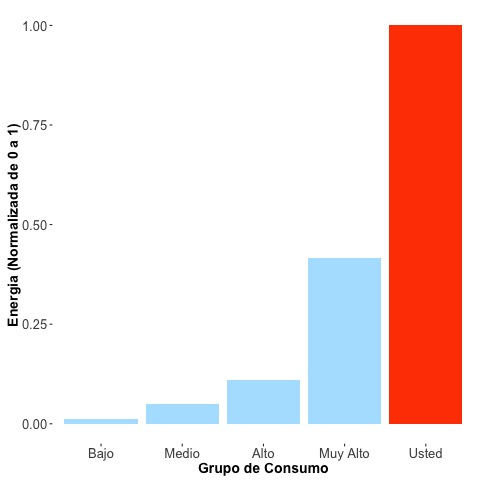
\includegraphics[scale=0.65]{figure/A1_neighbor_plot} 
\end{knitrout}

 \begin{textblock}{1}(9,-5)
\begin{minipage}{20em}
\begingroup
\input{A1_neighbor_plot.txt}
\endgroup
\end{minipage}
\end{textblock}

\begin{knitrout}
\definecolor{shadecolor}{rgb}{0.969, 0.969, 0.969}\color{fgcolor}
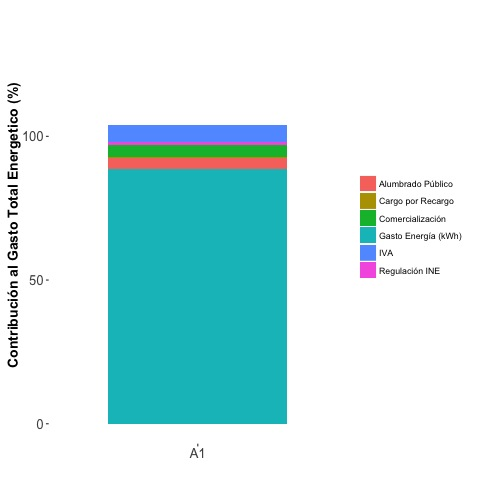
\includegraphics[scale=0.65]{figure/A1_costvars_plot.jpg} 
\end{knitrout}

 \begin{textblock}{1}(9,-5)
\begin{minipage}{20em}
\begingroup
\input{A1_costvars_plot.txt}
\endgroup
\end{minipage}
\end{textblock}

\begin{knitrout}
\definecolor{shadecolor}{rgb}{0.969, 0.969, 0.969}\color{fgcolor}
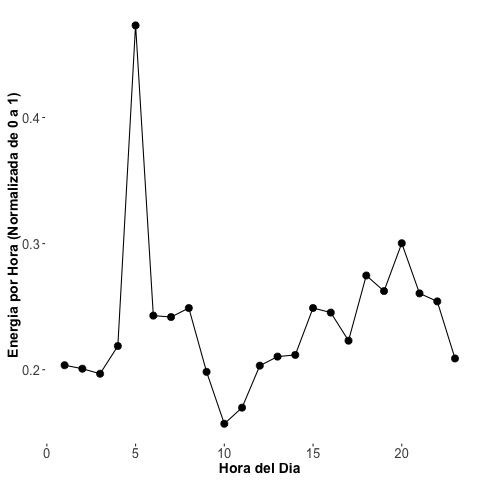
\includegraphics[scale=0.65]{figure/A1_plot_norm_median} 
\end{knitrout}


 \begin{textblock}{1}(9,-4)
\begin{minipage}{20em}
\begingroup
\input{A1_plot_norm_median.txt}
\endgroup
\end{minipage}
\end{textblock}


\begin{knitrout}
\definecolor{shadecolor}{rgb}{0.969, 0.969, 0.969}\color{fgcolor}
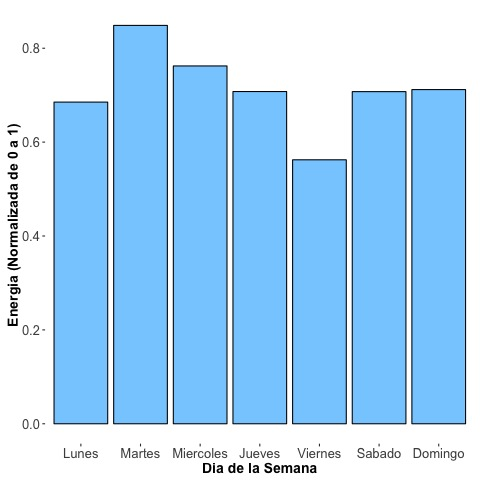
\includegraphics[scale=0.65]{figure/A1_day_of_week_plot} 
\end{knitrout}


 \begin{textblock}{1}(9,-3)
\begin{minipage}{20em}
\begingroup
\input{A1_day_of_week_plot.txt}
\endgroup
\end{minipage}
\end{textblock}

 \vspace{2cm}

\begin{knitrout}
\definecolor{shadecolor}{rgb}{0.969, 0.969, 0.969}\color{fgcolor}
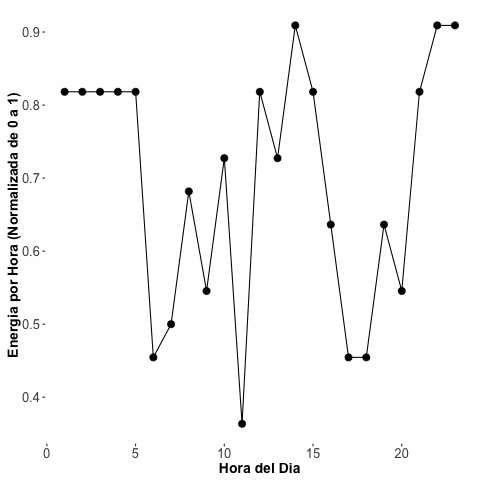
\includegraphics[scale=0.75]{figure/A1_fplot_norm_median} 
\end{knitrout}


 \begin{textblock}{1}(9,-4)
\begin{minipage}{20em}
\begingroup
\input{A1_fplot_norm_median.txt}
\endgroup
\end{minipage}
\end{textblock}

 \vspace{2cm}

\begin{knitrout}
\definecolor{shadecolor}{rgb}{0.969, 0.969, 0.969}\color{fgcolor}
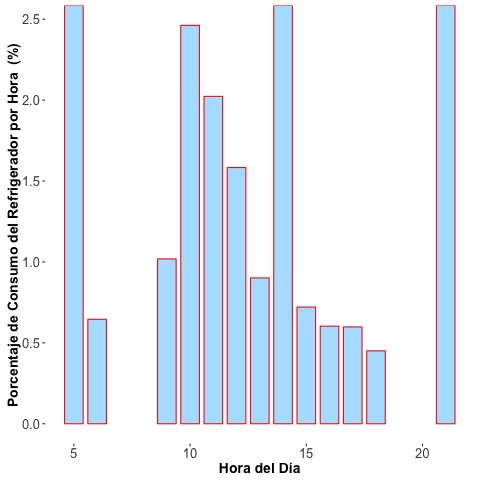
\includegraphics[scale=0.65]{figure/A1_fridge_energy_pct.jpg} 
\end{knitrout}

 \begin{textblock}{1}(9,-4)
\begin{minipage}{20em}
\begingroup
\input{A1_fridge_energy_pct.txt}
\endgroup
\end{minipage}
\end{textblock}


\begin{knitrout}
\definecolor{shadecolor}{rgb}{0.969, 0.969, 0.969}\color{fgcolor}
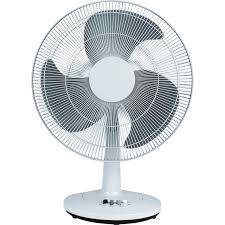
\includegraphics[scale=0.5]{figure/stock_fan.jpeg} 
\end{knitrout}

\begin{flushleft}
Un abanico es un electromestico muy comun en Managua. El abanico utiliza un motor para hacer girar unas aspas para mover el aire dentro de un cuarto. Uno calcula la energia y costo de un abanico de la siguiente manera: \newline

\textbf{ Energia al Dia (Watt-hora)} = Horas del uso Abanico por Dia  (Horas) x Consumo de Potencia (Watts)  \newline
\textbf{Cordobas al Dia}  = Horas del uso Abanico por Dia  (Horas) x Consumo de Potencia (Watts) x Costo de la energia (Cordobas/kWh) x (1000)
\end{flushleft}

\begin{knitrout}
\definecolor{shadecolor}{rgb}{0.969, 0.969, 0.969}\color{fgcolor}
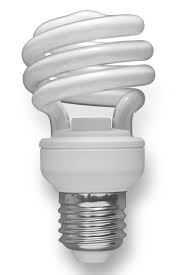
\includegraphics[scale=0.5]{figure/stock_light.jpeg} 
\end{knitrout}

\begin{flushleft}
Un foco CFL utiliza 1/3 o 1/5 de la energia que consume un foco incandescente. Los focos CFL son mas eficientes que los focos incandescentes. La cantidad de energia que consume un foco se calcula de la misma manera que lo que hicimos arriba para un abanico. \newline

\textbf{ Energia al Dia (Watt-hora)} = Horas con el foco Prendido por Dia  (Horas) x Consumo de Potencia (Watts)  \newline
\textbf{Cordobas al Dia}  = Horas con el uso foco Prendido por Dia  (Horas) x Consumo de Potencia (Watts) x Costo de la energia (Cordobas/kWh) x (1000)
\end{flushleft}

\begin{knitrout}
\definecolor{shadecolor}{rgb}{0.969, 0.969, 0.969}\color{fgcolor}

\includegraphics[scale=0.5]{figure/stock_freezer.jpeg} 
\end{knitrout}

\begin{flushleft}
El refrigerador consume energia solamente cuando el compresor esta prendido. Aunque la mantenedora o refrigerador esten conectados, estos solo consumiran energia cuando esten enfriando. Uno puede escuchar o sentir cuando los aparatos estan trabajando en enfriar el espacio dentro del refrigerado. Cuando el freezer o la mantenedora consumen energia, el consumo energetico y el gasto energetico se calculan de la misma manera que lo explicamos arriba. \newline

\textbf{ Energia al Dia (Watt-hora)} = Horas con el compresor prendido (o enfriando) por Dia  (Horas) x Consumo de Potencia (Watts)  \newline
\textbf{Cordobas al Dia}  = Horas con el compresor prendido (o enfriando)  por Dia  (Horas) x Consumo de Potencia (Watts) x Costo de la energia (Cordobas/kWh) x (1000)
\end{flushleft}

 \vspace{20cm}

\begin{flushleft}
\textbf{ TIPS PARA HACER A SU REFRIGERADOR O MANTENEDORA MAS EFICIENTE} \newline
\end{flushleft}

\begin{knitrout}
\definecolor{shadecolor}{rgb}{0.969, 0.969, 0.969}\color{fgcolor}
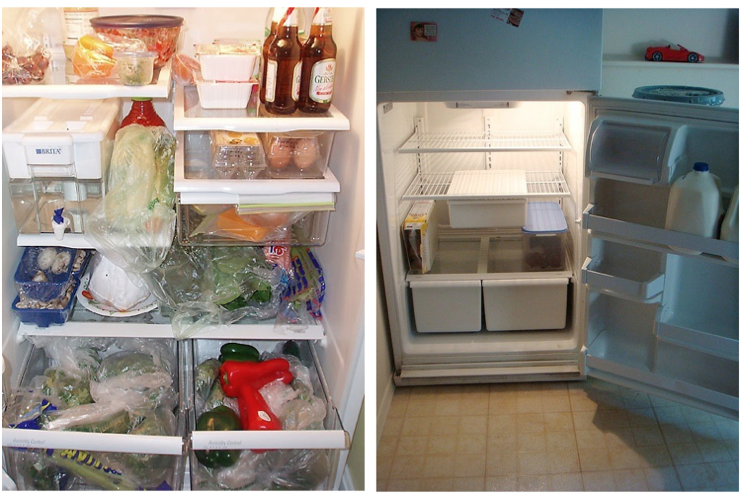
\includegraphics[scale=0.35]{figure/stock_fridgeefficiency1.png} 
\end{knitrout}

\begin{flushleft}
\textbf{1. Mantenga su Refrigerador o Mantenedora tan Lleno Como Pueda Durante el Dia y la Noche} \newline
Su refrigerador o mantenedora utiliza mucha energia para remplazar aire caliente con aire frio. Al mantener su refrigerador lleno su refrigerador gasta menos energia en enfriar el aire durante el dia y ademas los productos del refrigerador se mantienen frios mas tiempo. Usted puede congelar o meter bolsas o baldes de agua (cerrados) a su refrigerador o mantenedora para que este funcione mas eficientemente. Mientras mas lleno este su refrigerador, mejor funcionara.
\end{flushleft}

\begin{knitrout}
\definecolor{shadecolor}{rgb}{0.969, 0.969, 0.969}\color{fgcolor}
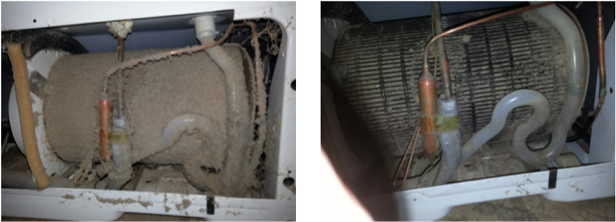
\includegraphics[scale=0.5]{figure/stock_condenser.png} 
\end{knitrout}

\begin{flushleft}
\textbf{2. Limpie el Condensador 2 a 3 Veces al Ano} \newline
Las bobinas del condensador (y el condensador) que mantienen a su refrigerador frio estan usualmente debajo o atras del refrigerador. Si estas tienen much polvo entonces impiden que circule el aire y hacen que el aparato tenga que trabajar mas que lo normal.  Se estima que el refrigerador puede ahorrar hasta el 15\% de su consumo energetico si uno mantiene el condensador y las bobinas limpias!
\end{flushleft}

\begin{knitrout}
\definecolor{shadecolor}{rgb}{0.969, 0.969, 0.969}\color{fgcolor}
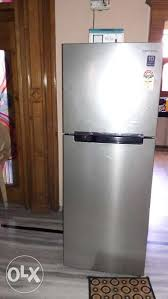
\includegraphics[scale=0.5]{figure/stock_space.jpeg} 
\end{knitrout}

\begin{flushleft}
\textbf{3. Mantenga buen Espacio entre el Refrigerador y las Paredes} \newline
Si usted tiene muy pegado su refrigerador a las paredes asegurase de separarlo. De igual manera, no ponga muchas cosas arriba de su refrigerador, o en los lados. Si mantiene muchas cosas arriba o a los lados del refrigerador entonces usted puede estar evitando que el refrigerador deseche todo el calor que esta generando.
\end{flushleft}

\begin{knitrout}
\definecolor{shadecolor}{rgb}{0.969, 0.969, 0.969}\color{fgcolor}
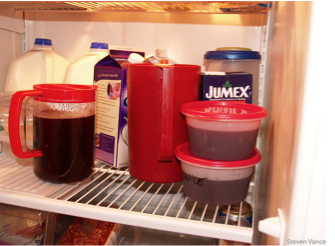
\includegraphics[scale=0.65]{figure/stock_lids.png} 
\end{knitrout}

\begin{flushleft}
\textbf{4. No Guarde Cosas Calientes o Cosas Descubiertas al Refrigerador} \newline
Si usted tiene algo caliente, espere a que se enfrie antes de meterlo al refrigerador. De igual manera, no guarde baldes o otras cosas que esten descubiertas. Meter cosas descubiertas crea humedad dentro del refrigerador que puede hacer que el compresor trabaje mas fuertemente. Asegurese que todo este frio y cerrado antes de meterlo al refrigerador. 
\end{flushleft}

\begin{knitrout}
\definecolor{shadecolor}{rgb}{0.969, 0.969, 0.969}\color{fgcolor}

\includegraphics[scale=0.65]{figure/stock_peek.png} 
\end{knitrout}

\begin{flushleft}
\textbf{5. No Abra la Puerta por Mucho Tiempo!} \newline
El abrir y cerrar de la puerta puede causar que el refrigerador consuma 50-120 kWh por ano! Asegurese de hacer el abrir y el cerrar de su refrigerador o mantenedora muy rapidamente.
\end{flushleft}

\begin{knitrout}
\definecolor{shadecolor}{rgb}{0.969, 0.969, 0.969}\color{fgcolor}
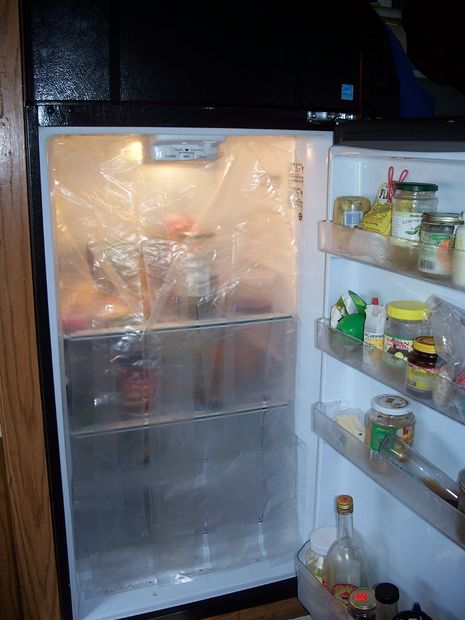
\includegraphics[scale=2]{figure/stock_doorinsulation.jpg} 
\end{knitrout}

\begin{flushleft}
\textbf{6. Construya una Puerta Interior de Plastico para Su Refrigerador} \newline
Utilizando algunas hojas de plastico transparente usted puede construir una puerta interior que funciona como insulacion. Usted cortaria esas hojas de plastico en tiras para poder ver lo que hay dentro del refrigerador, y poder pasar la mano a traves de las tiras de plastico sin permitir que el aire se salga. Debido a que el abrir y el cerrar de la puerta permite que el refrigerador o mantenedora se caliente, tener el plastico como barrera puede ahorrar mucha energia y costos relacionados al enfriamiento del refrigerador y/o mantenedora.
\end{flushleft}

\begin{knitrout}
\definecolor{shadecolor}{rgb}{0.969, 0.969, 0.969}\color{fgcolor}
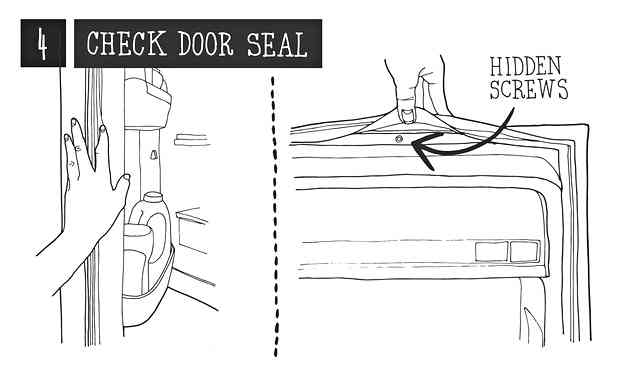
\includegraphics[scale=0.5]{figure/stock_seal.jpg} 
\end{knitrout}

\begin{flushleft}
\textbf{7. Selle o Reemplace el Plastico Alrededor de la Puerta de su Refrigerador} \newline
Aunque parezca que su refrigerador o mantenedora no tenga problemas, puede ser que pequeno hoyos en el sello de la puerta o el pl�stico permitan que aire fr�o salga y que aire caliente entre al refrigerador. El aire caliente se condensa r�pidamente y se congela que causa que se congele en partes del refrigerador donde no es deseable. Esto hace que el compresor este prendido mucho mas tiempo que lo que es necesario que incrementa el consumo energ�tico y el costo. Usted puede encontrar mas informaci�n al respecto aqu�: http://www.theguardian.com/lifeandstyle/2014/jul/21/how-to-mend-an-inefficient-fridge 
\end{flushleft}

 \vspace{2cm}

\begin{flushleft}
\textbf{SUGERENCIA PARA MEJORAR EL USO DE LUZ DURANTE EL DIA SIN ELECTRICIDAD} \newline
\end{flushleft}

\begin{knitrout}
\definecolor{shadecolor}{rgb}{0.969, 0.969, 0.969}\color{fgcolor}
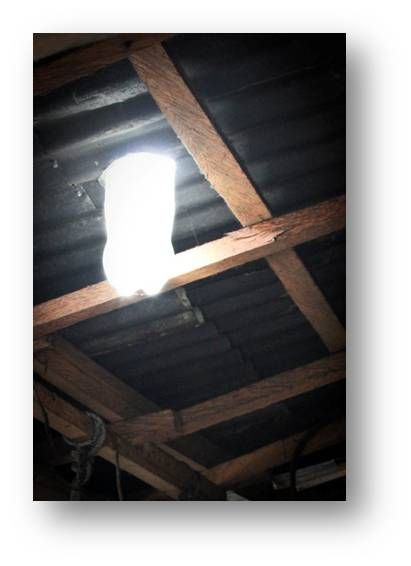
\includegraphics[scale=1]{figure/stock_bottle2.jpg} 
\end{knitrout}

\begin{flushleft}
\textbf{1. Materiales que Necesitara para La Lampara de Agua Luz} \newline
Para llevar acabo este ejercicio usted necesitara una botella de pl�stico de 1.5 o 2 L, sellador, un pedazo de lamina de metal para techo, agua limpia, y blanqueador. 
\end{flushleft}

\begin{knitrout}
\definecolor{shadecolor}{rgb}{0.969, 0.969, 0.969}\color{fgcolor}
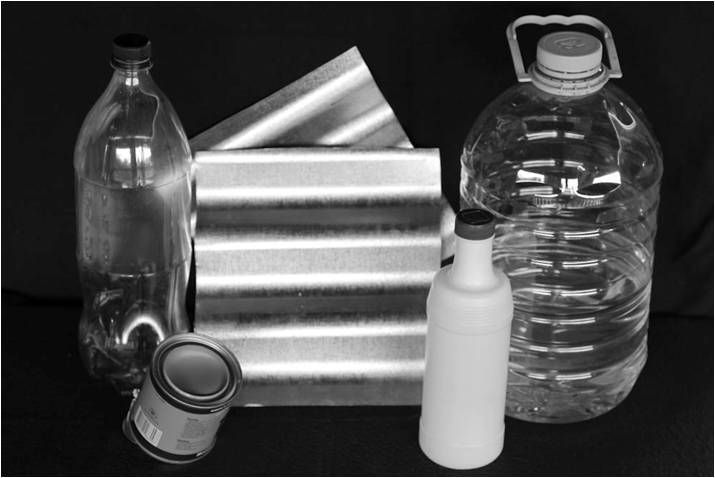
\includegraphics[scale=1]{figure/stock_equipment.jpg} 
\end{knitrout}

\begin{flushleft}
\textbf{2. Corte Aproximadamente 25 x 25 cm de Lamina Corrugada o Plana (Depende de su Techo) }
\end{flushleft}

\begin{knitrout}
\definecolor{shadecolor}{rgb}{0.969, 0.969, 0.969}\color{fgcolor}
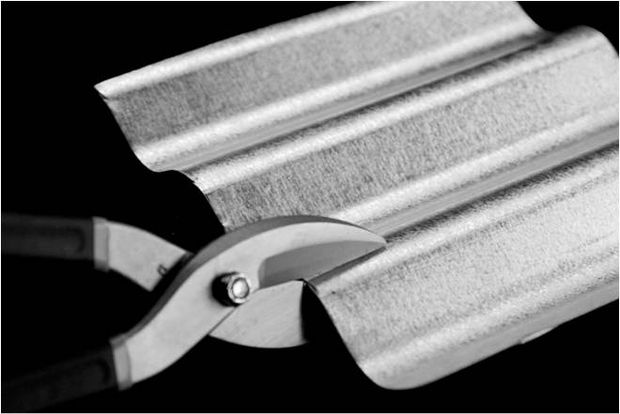
\includegraphics[scale=1]{figure/stock_bottle3.jpg} 
\end{knitrout}

\begin{flushleft}
\textbf{3. En el Centro de la Lamina Dibuje dos Circulos de Tamano suficiente para que se Atore la Parte Gorda de la Botella }
\end{flushleft}

\begin{knitrout}
\definecolor{shadecolor}{rgb}{0.969, 0.969, 0.969}\color{fgcolor}
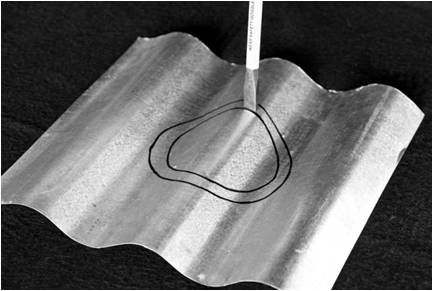
\includegraphics[scale=1.5]{figure/stock_bottle4.jpg} 
\end{knitrout}

\begin{flushleft}
\textbf{4. Corte la Diferencia entre las Dos Lineas (1 cm), haga tiritas, y voltee las tiritas para arriba para que est�n perpendiculares a la lamina}
\end{flushleft}

\begin{knitrout}
\definecolor{shadecolor}{rgb}{0.969, 0.969, 0.969}\color{fgcolor}
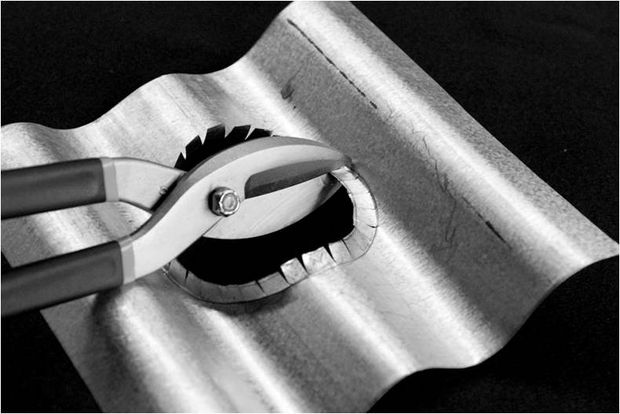
\includegraphics[scale=1]{figure/stock_bottle5.jpg} 
\end{knitrout}

\begin{flushleft}
\textbf{5. Utilize papel de lija para limpiar la botella en el area que se va a pegar a la lamina para que el sellador pegue mejor}
\end{flushleft}

\begin{knitrout}
\definecolor{shadecolor}{rgb}{0.969, 0.969, 0.969}\color{fgcolor}
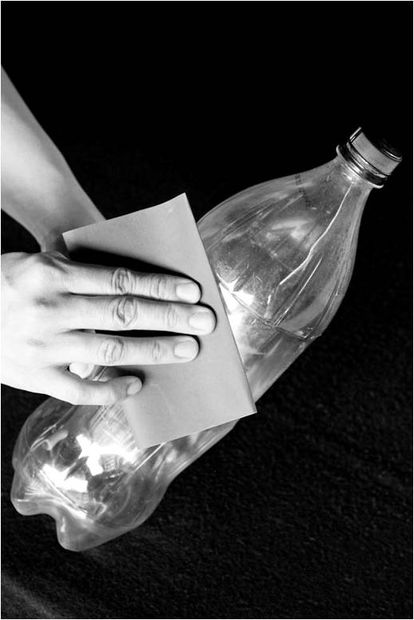
\includegraphics[scale=1]{figure/stock_bottle6.jpg} 
\end{knitrout}

\begin{flushleft}
\textbf{6. Meta la botella a la lamina hasta la ultima parte. Aplique el sellador arriba de las tiritas y alrededor del area abajo de la botella. Espere a que se seque.}
\end{flushleft}

\begin{knitrout}
\definecolor{shadecolor}{rgb}{0.969, 0.969, 0.969}\color{fgcolor}
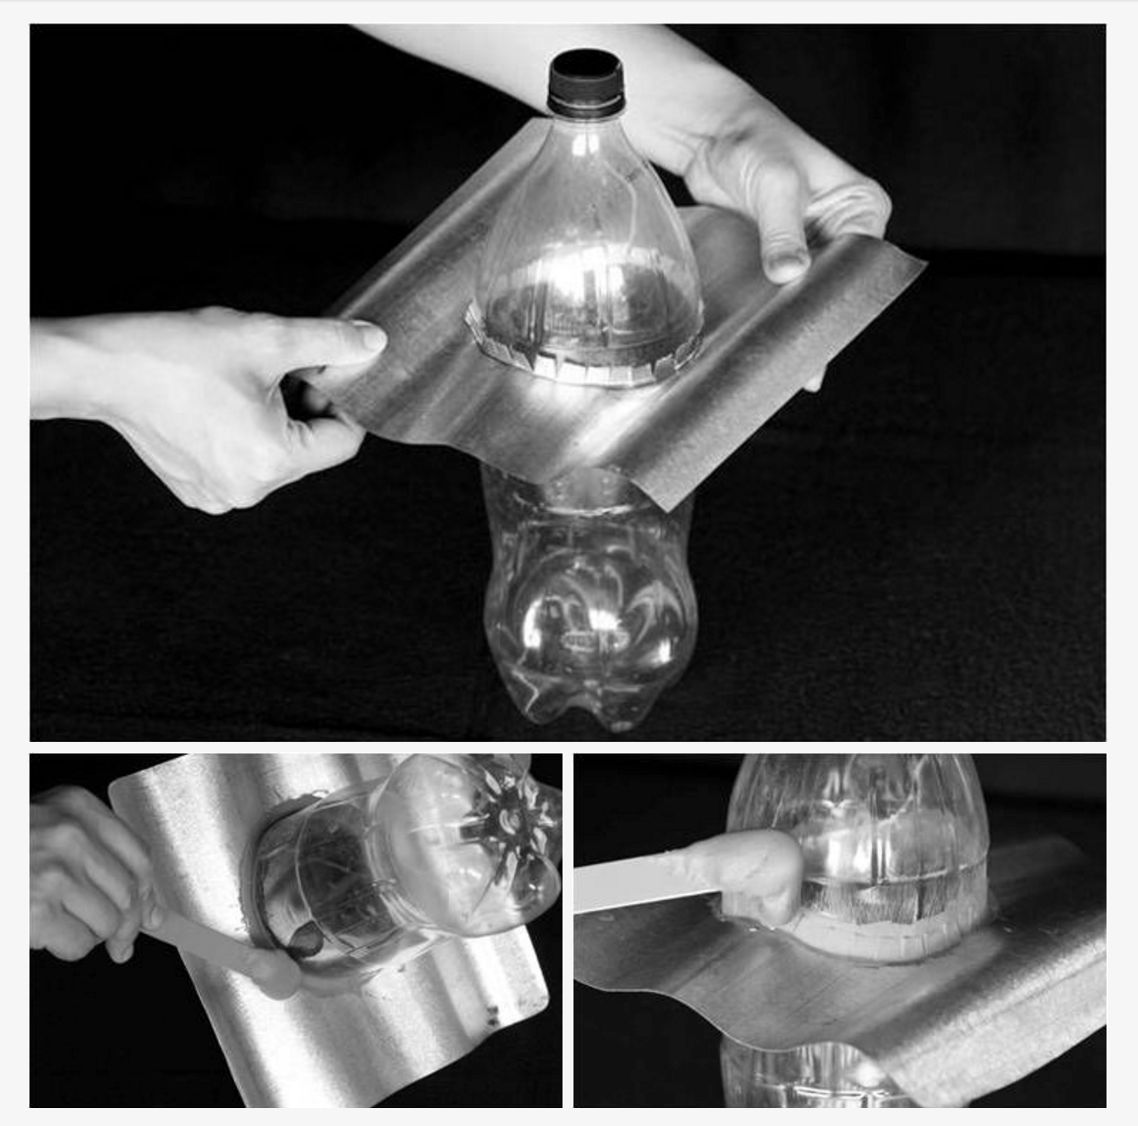
\includegraphics[scale=0.45]{figure/stock_bottle7.jpg} 
\end{knitrout}

\begin{flushleft}
\textbf{7. Llene la botella con agua limpia (de filtro) y aproximadamente 10 mililitros de blanqueador. Cierre la botella.}
\end{flushleft}

\begin{knitrout}
\definecolor{shadecolor}{rgb}{0.969, 0.969, 0.969}\color{fgcolor}
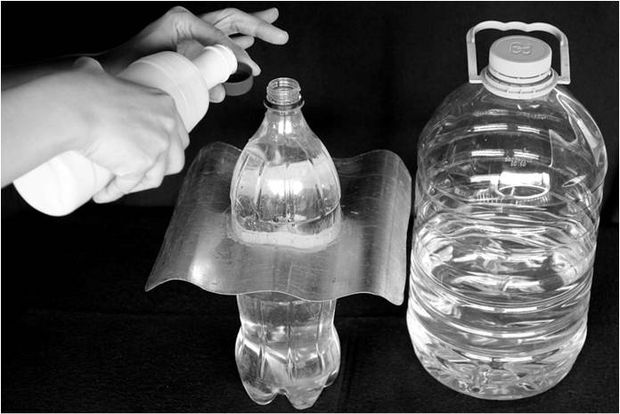
\includegraphics[scale=1]{figure/stock_bottle8.jpg} 
\end{knitrout}

\begin{flushleft}
\textbf{8. Instale la lamina con la botella en su techo. Ponga sellador en todos lados. Espere a que seque. Si hace falta, utilize clavos o un taladro para asegurar la pieza bien al techo}
\end{flushleft}

\begin{knitrout}
\definecolor{shadecolor}{rgb}{0.969, 0.969, 0.969}\color{fgcolor}
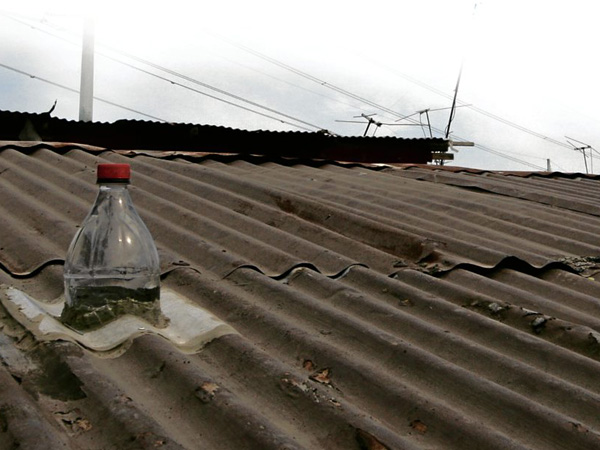
\includegraphics[scale=0.45]{figure/stock_bottle9.jpg} 
\end{knitrout}

\begin{flushleft}
\textbf{9. AHORA USTED TIENE UNA LAMPARA DE AGUA Y LUZ QUE NO USA ELECTRICIDAD DURANTE EL DIA!!!}
\end{flushleft}

\begin{knitrout}
\definecolor{shadecolor}{rgb}{0.969, 0.969, 0.969}\color{fgcolor}
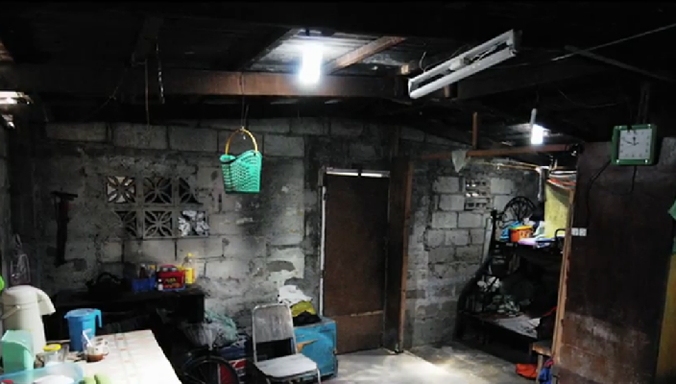
\includegraphics[scale=0.75]{figure/stock_bottle10.png} 
\end{knitrout}


 \vspace{20cm}


\begin{knitrout}
\definecolor{shadecolor}{rgb}{0.969, 0.969, 0.969}\color{fgcolor}
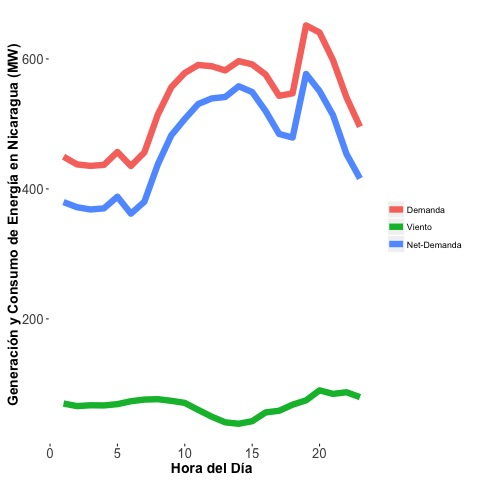
\includegraphics[scale=0.65]{figure/gridplot1.jpg} 
\end{knitrout}

 \begin{textblock}{1}(9,-5)
\begin{minipage}{20em}
\begingroup
\input{grid_text1.txt}
\endgroup
\end{minipage}
\end{textblock}

 \vspace{2cm}

\begin{knitrout}
\definecolor{shadecolor}{rgb}{0.969, 0.969, 0.969}\color{fgcolor}
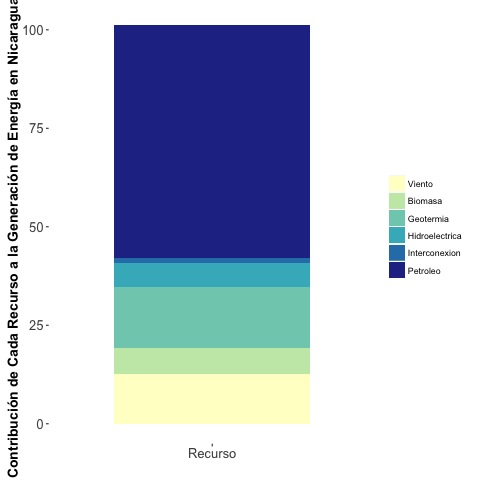
\includegraphics[scale=0.65]{figure/gridplot2.jpg} 
\end{knitrout}

 \begin{textblock}{1}(9,-5)
\begin{minipage}{20em}
\begingroup
\input{grid_text2.txt}
\endgroup
\end{minipage}
\end{textblock}

\begin{knitrout}
\definecolor{shadecolor}{rgb}{0.969, 0.969, 0.969}\color{fgcolor}
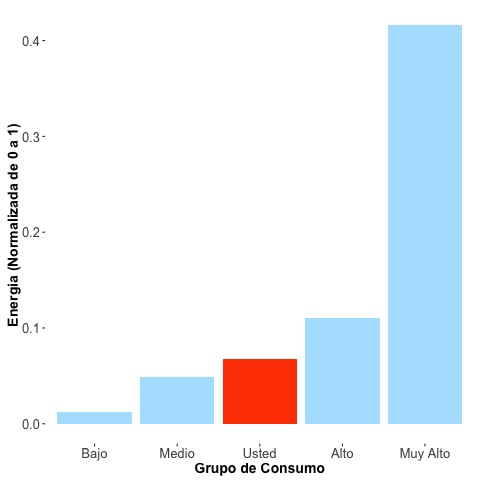
\includegraphics[scale=0.65]{figure/A3_neighbor_plot} 
\end{knitrout}

 \begin{textblock}{1}(9,-5)
\begin{minipage}{20em}
\begingroup
\input{A3_neighbor_plot.txt}
\endgroup
\end{minipage}
\end{textblock}

\begin{knitrout}
\definecolor{shadecolor}{rgb}{0.969, 0.969, 0.969}\color{fgcolor}
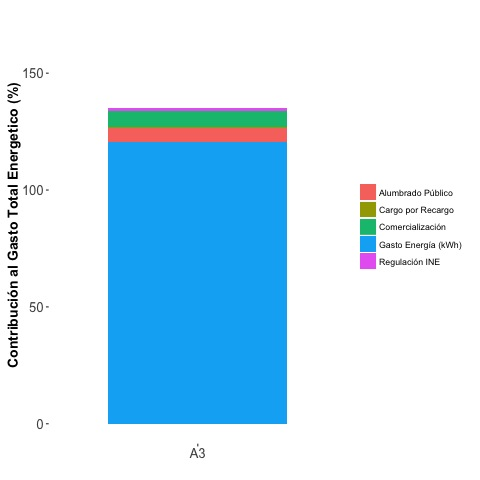
\includegraphics[scale=0.65]{figure/A3_costvars_plot.jpg} 
\end{knitrout}

 \begin{textblock}{1}(9,-5)
\begin{minipage}{20em}
\begingroup
\input{A3_costvars_plot.txt}
\endgroup
\end{minipage}
\end{textblock}

\begin{knitrout}
\definecolor{shadecolor}{rgb}{0.969, 0.969, 0.969}\color{fgcolor}
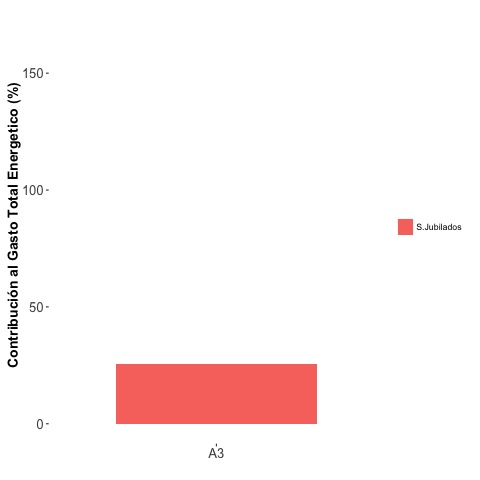
\includegraphics[scale=0.65]{figure/A3_subvars_plot.jpg} 
\end{knitrout}

 \begin{textblock}{1}(9,-5)
\begin{minipage}{20em}
\begingroup
\input{A3_subvars_plot.txt}
\endgroup
\end{minipage}
\end{textblock}

\begin{knitrout}
\definecolor{shadecolor}{rgb}{0.969, 0.969, 0.969}\color{fgcolor}
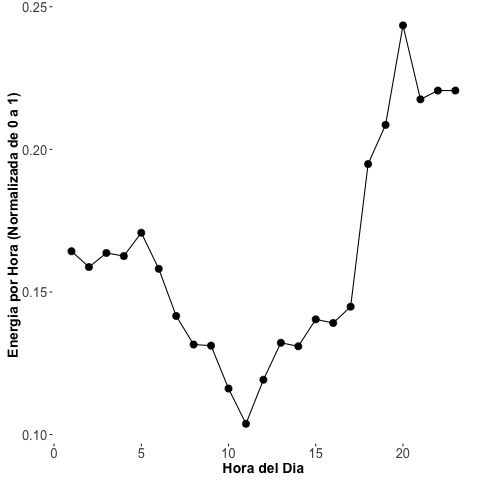
\includegraphics[scale=0.65]{figure/A3_plot_norm_median} 
\end{knitrout}


 \begin{textblock}{1}(9,-4)
\begin{minipage}{20em}
\begingroup
\input{A3_plot_norm_median.txt}
\endgroup
\end{minipage}
\end{textblock}


\begin{knitrout}
\definecolor{shadecolor}{rgb}{0.969, 0.969, 0.969}\color{fgcolor}
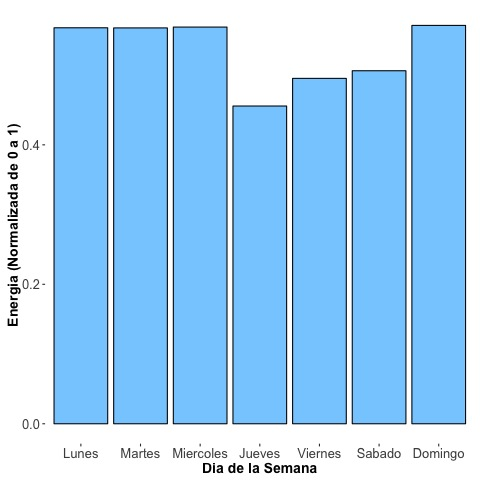
\includegraphics[scale=0.65]{figure/A3_day_of_week_plot} 
\end{knitrout}


 \begin{textblock}{1}(9,-3)
\begin{minipage}{20em}
\begingroup
\input{A3_day_of_week_plot.txt}
\endgroup
\end{minipage}
\end{textblock}

 \vspace{2cm}

\begin{knitrout}
\definecolor{shadecolor}{rgb}{0.969, 0.969, 0.969}\color{fgcolor}
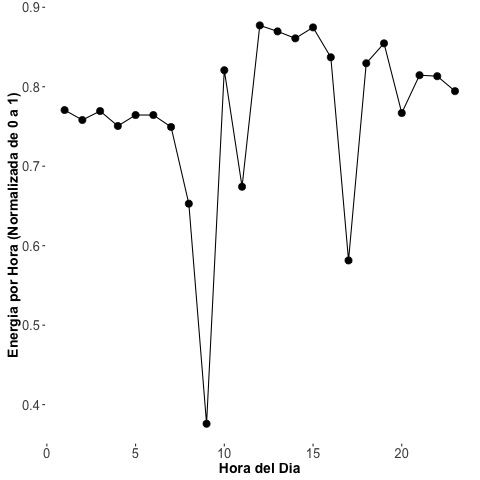
\includegraphics[scale=0.75]{figure/A3_fplot_norm_median} 
\end{knitrout}


 \begin{textblock}{1}(9,-4)
\begin{minipage}{20em}
\begingroup
\input{A3_fplot_norm_median.txt}
\endgroup
\end{minipage}
\end{textblock}

 \vspace{2cm}

\begin{knitrout}
\definecolor{shadecolor}{rgb}{0.969, 0.969, 0.969}\color{fgcolor}
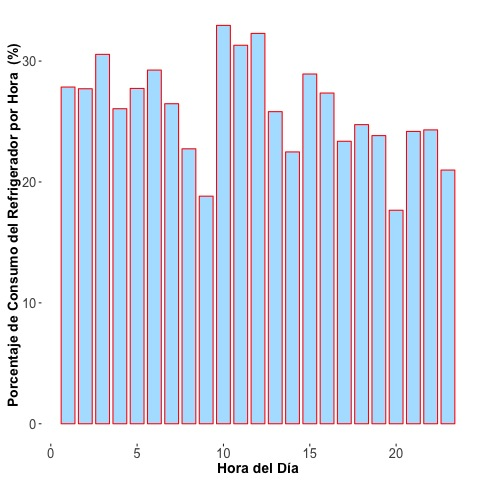
\includegraphics[scale=0.65]{figure/A3_fridge_energy_pct.jpg} 
\end{knitrout}

 \begin{textblock}{1}(9,-4)
\begin{minipage}{20em}
\begingroup
\input{A3_fridge_energy_pct.txt}
\endgroup
\end{minipage}
\end{textblock}

 \vspace{20cm}
 

\begin{knitrout}
\definecolor{shadecolor}{rgb}{0.969, 0.969, 0.969}\color{fgcolor}
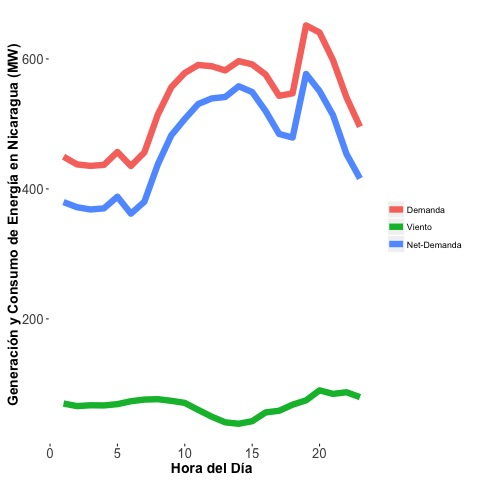
\includegraphics[scale=0.65]{figure/gridplot1.jpg} 
\end{knitrout}

 \begin{textblock}{1}(9,-5)
\begin{minipage}{20em}
\begingroup
\input{grid_text1.txt}
\endgroup
\end{minipage}
\end{textblock}

 \vspace{2cm}

\begin{knitrout}
\definecolor{shadecolor}{rgb}{0.969, 0.969, 0.969}\color{fgcolor}
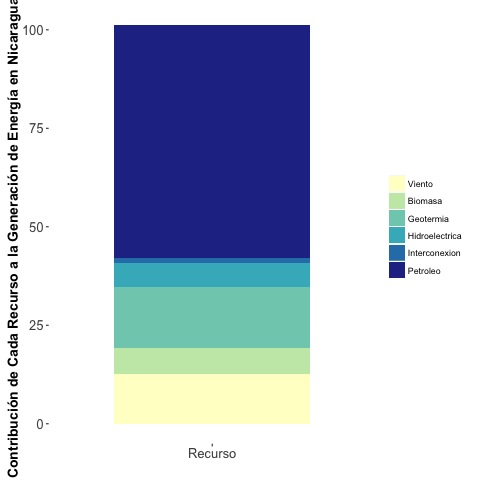
\includegraphics[scale=0.65]{figure/gridplot2.jpg} 
\end{knitrout}

 \begin{textblock}{1}(9,-5)
\begin{minipage}{20em}
\begingroup
\input{grid_text2.txt}
\endgroup
\end{minipage}
\end{textblock}

\begin{knitrout}
\definecolor{shadecolor}{rgb}{0.969, 0.969, 0.969}\color{fgcolor}
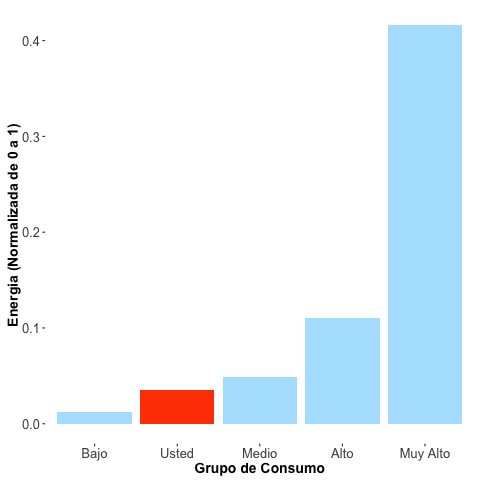
\includegraphics[scale=0.65]{figure/A6_neighbor_plot} 
\end{knitrout}

 \begin{textblock}{1}(9,-5)
\begin{minipage}{20em}
\begingroup
\input{A6_neighbor_plot.txt}
\endgroup
\end{minipage}
\end{textblock}

\begin{knitrout}
\definecolor{shadecolor}{rgb}{0.969, 0.969, 0.969}\color{fgcolor}
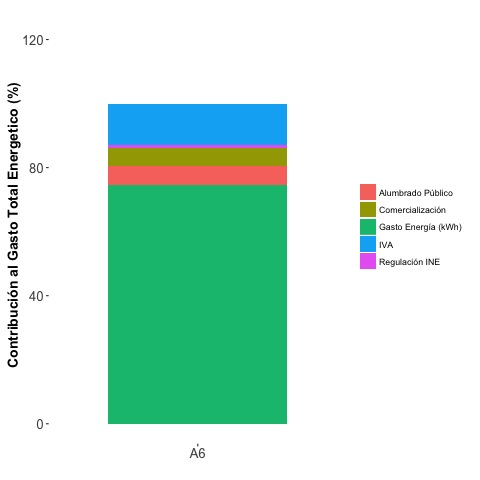
\includegraphics[scale=0.65]{figure/A6_costvars_plot.jpg} 
\end{knitrout}

 \begin{textblock}{1}(9,-5)
\begin{minipage}{20em}
\begingroup
\input{A6_costvars_plot.txt}
\endgroup
\end{minipage}
\end{textblock}

\begin{knitrout}
\definecolor{shadecolor}{rgb}{0.969, 0.969, 0.969}\color{fgcolor}
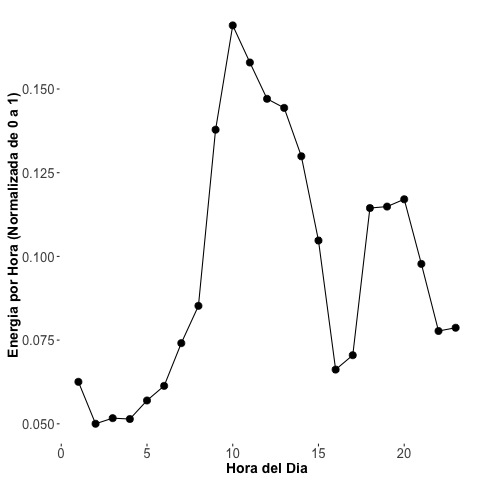
\includegraphics[scale=0.65]{figure/A6_plot_norm_median} 
\end{knitrout}


 \begin{textblock}{1}(9,-4)
\begin{minipage}{20em}
\begingroup
\input{A6_plot_norm_median.txt}
\endgroup
\end{minipage}
\end{textblock}


\begin{knitrout}
\definecolor{shadecolor}{rgb}{0.969, 0.969, 0.969}\color{fgcolor}
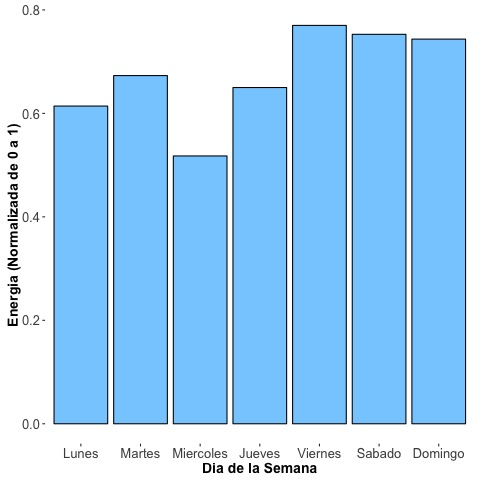
\includegraphics[scale=0.65]{figure/A6_day_of_week_plot} 
\end{knitrout}


 \begin{textblock}{1}(9,-3)
\begin{minipage}{20em}
\begingroup
\input{A6_day_of_week_plot.txt}
\endgroup
\end{minipage}
\end{textblock}

 \vspace{2cm}

\begin{knitrout}
\definecolor{shadecolor}{rgb}{0.969, 0.969, 0.969}\color{fgcolor}
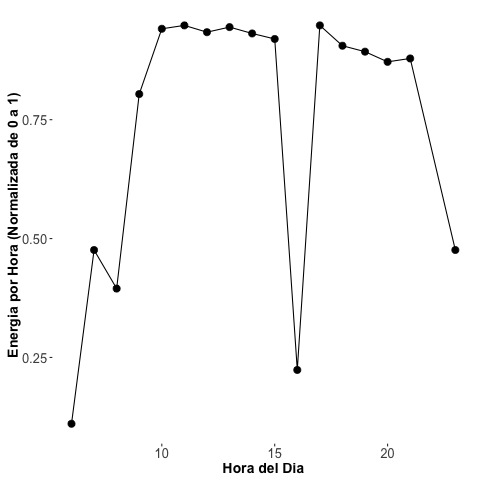
\includegraphics[scale=0.75]{figure/A6_fplot_norm_median} 
\end{knitrout}


 \begin{textblock}{1}(9,-4)
\begin{minipage}{20em}
\begingroup
\input{A6_fplot_norm_median.txt}
\endgroup
\end{minipage}
\end{textblock}

 \vspace{2cm}

\begin{knitrout}
\definecolor{shadecolor}{rgb}{0.969, 0.969, 0.969}\color{fgcolor}
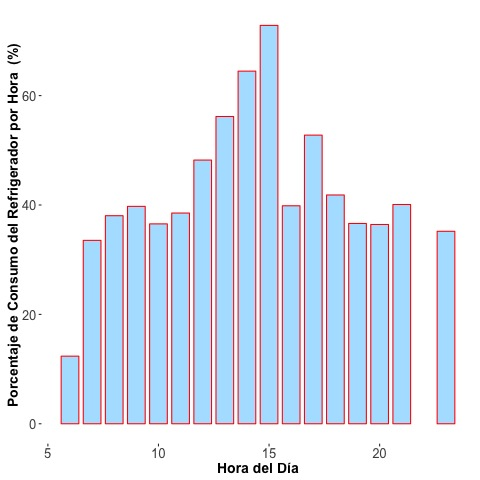
\includegraphics[scale=0.65]{figure/A6_fridge_energy_pct.jpg} 
\end{knitrout}

 \begin{textblock}{1}(9,-4)
\begin{minipage}{20em}
\begingroup
\input{A6_fridge_energy_pct.txt}
\endgroup
\end{minipage}
\end{textblock}

\vspace{20cm}
 

\begin{knitrout}
\definecolor{shadecolor}{rgb}{0.969, 0.969, 0.969}\color{fgcolor}
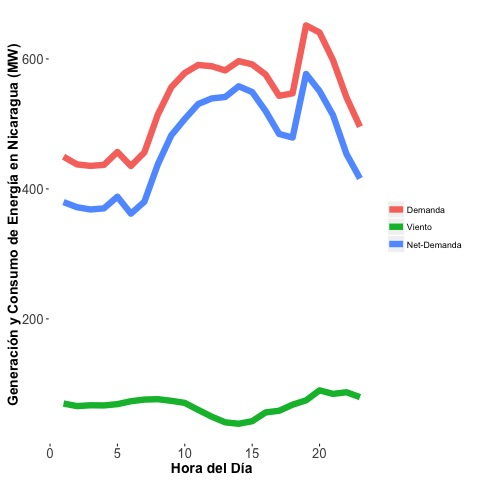
\includegraphics[scale=0.65]{figure/gridplot1.jpg} 
\end{knitrout}

 \begin{textblock}{1}(9,-5)
\begin{minipage}{20em}
\begingroup
\input{grid_text1.txt}
\endgroup
\end{minipage}
\end{textblock}

 \vspace{2cm}

\begin{knitrout}
\definecolor{shadecolor}{rgb}{0.969, 0.969, 0.969}\color{fgcolor}
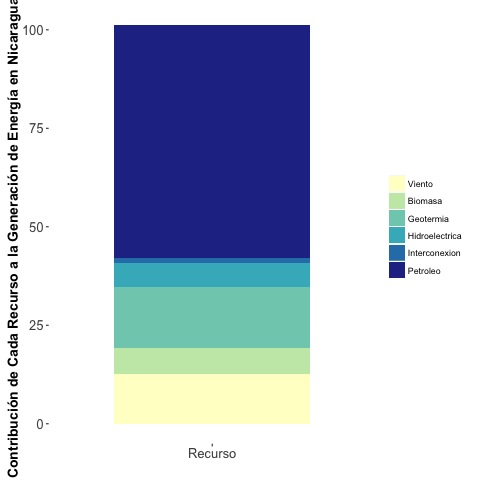
\includegraphics[scale=0.65]{figure/gridplot2.jpg} 
\end{knitrout}

 \begin{textblock}{1}(9,-5)
\begin{minipage}{20em}
\begingroup
\input{grid_text2.txt}
\endgroup
\end{minipage}
\end{textblock}

\begin{knitrout}
\definecolor{shadecolor}{rgb}{0.969, 0.969, 0.969}\color{fgcolor}
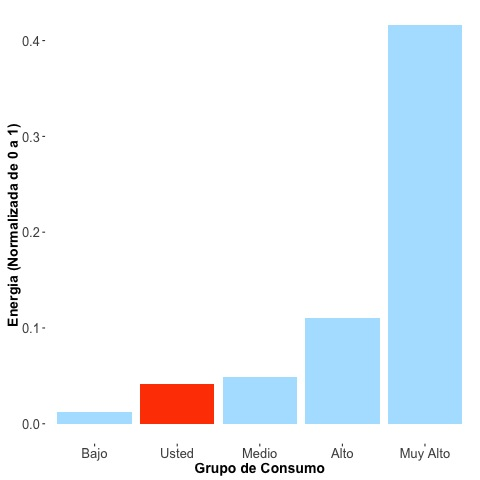
\includegraphics[scale=0.65]{figure/A7_neighbor_plot} 
\end{knitrout}

 \begin{textblock}{1}(9,-5)
\begin{minipage}{20em}
\begingroup
\input{A7_neighbor_plot.txt}
\endgroup
\end{minipage}
\end{textblock}

\begin{knitrout}
\definecolor{shadecolor}{rgb}{0.969, 0.969, 0.969}\color{fgcolor}
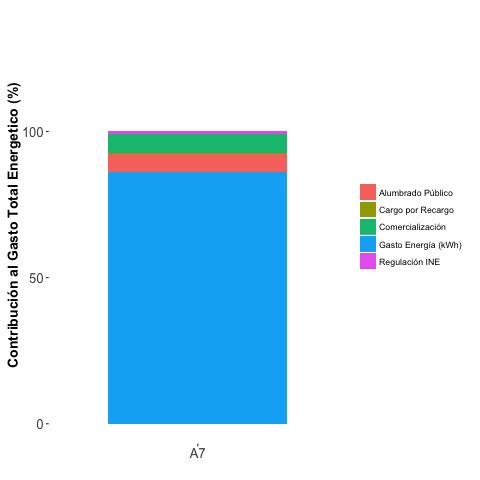
\includegraphics[scale=0.65]{figure/A7_costvars_plot.jpg} 
\end{knitrout}

 \begin{textblock}{1}(9,-5)
\begin{minipage}{20em}
\begingroup
\input{A7_costvars_plot.txt}
\endgroup
\end{minipage}
\end{textblock}

\begin{knitrout}
\definecolor{shadecolor}{rgb}{0.969, 0.969, 0.969}\color{fgcolor}
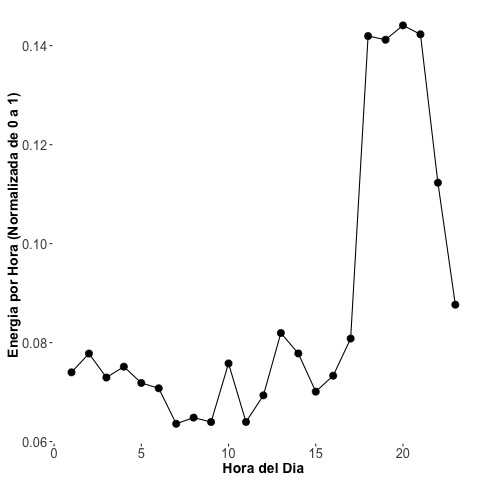
\includegraphics[scale=0.65]{figure/A7_plot_norm_median} 
\end{knitrout}


 \begin{textblock}{1}(9,-4)
\begin{minipage}{20em}
\begingroup
\input{A7_plot_norm_median.txt}
\endgroup
\end{minipage}
\end{textblock}


\begin{knitrout}
\definecolor{shadecolor}{rgb}{0.969, 0.969, 0.969}\color{fgcolor}
\includegraphics[scale=0.65]{figure/A7_day_of_week_plot} 
\end{knitrout}


 \begin{textblock}{1}(9,-3)
\begin{minipage}{20em}
\begingroup
\input{A7_day_of_week_plot.txt}
\endgroup
\end{minipage}
\end{textblock}

 \vspace{2cm}

\begin{knitrout}
\definecolor{shadecolor}{rgb}{0.969, 0.969, 0.969}\color{fgcolor}
\includegraphics[scale=0.75]{figure/A7_fplot_norm_median} 
\end{knitrout}


 \begin{textblock}{1}(9,-4)
\begin{minipage}{20em}
\begingroup
\input{A7_fplot_norm_median.txt}
\endgroup
\end{minipage}
\end{textblock}

 \vspace{2cm}

\begin{knitrout}
\definecolor{shadecolor}{rgb}{0.969, 0.969, 0.969}\color{fgcolor}
\includegraphics[scale=0.65]{figure/A7_fridge_energy_pct.jpg} 
\end{knitrout}

 \begin{textblock}{1}(9,-4)
\begin{minipage}{20em}
\begingroup
\input{A7_fridge_energy_pct.txt}
\endgroup
\end{minipage}
\end{textblock}

\vspace{20cm}
 

\begin{knitrout}
\definecolor{shadecolor}{rgb}{0.969, 0.969, 0.969}\color{fgcolor}
\includegraphics[scale=0.65]{figure/gridplot1.jpg} 
\end{knitrout}

 \begin{textblock}{1}(9,-5)
\begin{minipage}{20em}
\begingroup
\input{grid_text1.txt}
\endgroup
\end{minipage}
\end{textblock}

 \vspace{2cm}

\begin{knitrout}
\definecolor{shadecolor}{rgb}{0.969, 0.969, 0.969}\color{fgcolor}
\includegraphics[scale=0.65]{figure/gridplot2.jpg} 
\end{knitrout}

 \begin{textblock}{1}(9,-5)
\begin{minipage}{20em}
\begingroup
\input{grid_text2.txt}
\endgroup
\end{minipage}
\end{textblock}

\begin{knitrout}
\definecolor{shadecolor}{rgb}{0.969, 0.969, 0.969}\color{fgcolor}
\includegraphics[scale=0.65]{figure/A9_neighbor_plot} 
\end{knitrout}

 \begin{textblock}{1}(9,-5)
\begin{minipage}{20em}
\begingroup
\input{A9_neighbor_plot.txt}
\endgroup
\end{minipage}
\end{textblock}

\begin{knitrout}
\definecolor{shadecolor}{rgb}{0.969, 0.969, 0.969}\color{fgcolor}
\includegraphics[scale=0.65]{figure/A9_costvars_plot.jpg} 
\end{knitrout}

 \begin{textblock}{1}(9,-5)
\begin{minipage}{20em}
\begingroup
\input{A9_costvars_plot.txt}
\endgroup
\end{minipage}
\end{textblock}

\begin{knitrout}
\definecolor{shadecolor}{rgb}{0.969, 0.969, 0.969}\color{fgcolor}
\includegraphics[scale=0.65]{figure/A9_plot_norm_median} 
\end{knitrout}


 \begin{textblock}{1}(9,-4)
\begin{minipage}{20em}
\begingroup
\input{A9_plot_norm_median.txt}
\endgroup
\end{minipage}
\end{textblock}


\begin{knitrout}
\definecolor{shadecolor}{rgb}{0.969, 0.969, 0.969}\color{fgcolor}
\includegraphics[scale=0.65]{figure/A9_day_of_week_plot} 
\end{knitrout}


 \begin{textblock}{1}(9,-3)
\begin{minipage}{20em}
\begingroup
\input{A9_day_of_week_plot.txt}
\endgroup
\end{minipage}
\end{textblock}

 \vspace{2cm}

\begin{knitrout}
\definecolor{shadecolor}{rgb}{0.969, 0.969, 0.969}\color{fgcolor}
\includegraphics[scale=0.75]{figure/A9_fplot_norm_median} 
\end{knitrout}


 \begin{textblock}{1}(9,-4)
\begin{minipage}{20em}
\begingroup
\input{A9_fplot_norm_median.txt}
\endgroup
\end{minipage}
\end{textblock}

 \vspace{2cm}

\begin{knitrout}
\definecolor{shadecolor}{rgb}{0.969, 0.969, 0.969}\color{fgcolor}
\includegraphics[scale=0.65]{figure/A9_fridge_energy_pct.jpg} 
\end{knitrout}

 \begin{textblock}{1}(9,-4)
\begin{minipage}{20em}
\begingroup
\input{A9_fridge_energy_pct.txt}
\endgroup
\end{minipage}
\end{textblock}

\vspace{20cm}
 

\begin{knitrout}
\definecolor{shadecolor}{rgb}{0.969, 0.969, 0.969}\color{fgcolor}
\includegraphics[scale=0.65]{figure/gridplot1.jpg} 
\end{knitrout}

 \begin{textblock}{1}(9,-5)
\begin{minipage}{20em}
\begingroup
\input{grid_text1.txt}
\endgroup
\end{minipage}
\end{textblock}

 \vspace{2cm}

\begin{knitrout}
\definecolor{shadecolor}{rgb}{0.969, 0.969, 0.969}\color{fgcolor}
\includegraphics[scale=0.65]{figure/gridplot2.jpg} 
\end{knitrout}

 \begin{textblock}{1}(9,-5)
\begin{minipage}{20em}
\begingroup
\input{grid_text2.txt}
\endgroup
\end{minipage}
\end{textblock}

\begin{knitrout}
\definecolor{shadecolor}{rgb}{0.969, 0.969, 0.969}\color{fgcolor}
\includegraphics[scale=0.65]{figure/A11_neighbor_plot} 
\end{knitrout}

 \begin{textblock}{1}(9,-5)
\begin{minipage}{20em}
\begingroup
\input{A11_neighbor_plot.txt}
\endgroup
\end{minipage}
\end{textblock}

\begin{knitrout}
\definecolor{shadecolor}{rgb}{0.969, 0.969, 0.969}\color{fgcolor}
\includegraphics[scale=0.65]{figure/A11_costvars_plot.jpg} 
\end{knitrout}

 \begin{textblock}{1}(9,-5)
\begin{minipage}{20em}
\begingroup
\input{A11_costvars_plot.txt}
\endgroup
\end{minipage}
\end{textblock}

\begin{knitrout}
\definecolor{shadecolor}{rgb}{0.969, 0.969, 0.969}\color{fgcolor}
\includegraphics[scale=0.65]{figure/A11_plot_norm_median} 
\end{knitrout}


 \begin{textblock}{1}(9,-4)
\begin{minipage}{20em}
\begingroup
\input{A11_plot_norm_median.txt}
\endgroup
\end{minipage}
\end{textblock}


\begin{knitrout}
\definecolor{shadecolor}{rgb}{0.969, 0.969, 0.969}\color{fgcolor}
\includegraphics[scale=0.65]{figure/A11_day_of_week_plot} 
\end{knitrout}


 \begin{textblock}{1}(9,-3)
\begin{minipage}{20em}
\begingroup
\input{A11_day_of_week_plot.txt}
\endgroup
\end{minipage}
\end{textblock}

 \vspace{2cm}

\begin{knitrout}
\definecolor{shadecolor}{rgb}{0.969, 0.969, 0.969}\color{fgcolor}
\includegraphics[scale=0.75]{figure/A11_fplot_norm_median} 
\end{knitrout}


 \begin{textblock}{1}(9,-4)
\begin{minipage}{20em}
\begingroup
\input{A11_fplot_norm_median.txt}
\endgroup
\end{minipage}
\end{textblock}

 \vspace{2cm}

\begin{knitrout}
\definecolor{shadecolor}{rgb}{0.969, 0.969, 0.969}\color{fgcolor}
\includegraphics[scale=0.65]{figure/A11_fridge_energy_pct.jpg} 
\end{knitrout}

 \begin{textblock}{1}(9,-4)
\begin{minipage}{20em}
\begingroup
\input{A11_fridge_energy_pct.txt}
\endgroup
\end{minipage}
\end{textblock}

\vspace{20cm}
 

\begin{knitrout}
\definecolor{shadecolor}{rgb}{0.969, 0.969, 0.969}\color{fgcolor}
\includegraphics[scale=0.65]{figure/gridplot1.jpg} 
\end{knitrout}

 \begin{textblock}{1}(9,-5)
\begin{minipage}{20em}
\begingroup
\input{grid_text1.txt}
\endgroup
\end{minipage}
\end{textblock}

 \vspace{2cm}

\begin{knitrout}
\definecolor{shadecolor}{rgb}{0.969, 0.969, 0.969}\color{fgcolor}
\includegraphics[scale=0.65]{figure/gridplot2.jpg} 
\end{knitrout}

 \begin{textblock}{1}(9,-5)
\begin{minipage}{20em}
\begingroup
\input{grid_text2.txt}
\endgroup
\end{minipage}
\end{textblock}

\begin{knitrout}
\definecolor{shadecolor}{rgb}{0.969, 0.969, 0.969}\color{fgcolor}
\includegraphics[scale=0.65]{figure/A12_neighbor_plot} 
\end{knitrout}

 \begin{textblock}{1}(9,-5)
\begin{minipage}{20em}
\begingroup
\input{A12_neighbor_plot.txt}
\endgroup
\end{minipage}
\end{textblock}

\begin{knitrout}
\definecolor{shadecolor}{rgb}{0.969, 0.969, 0.969}\color{fgcolor}
\includegraphics[scale=0.65]{figure/A12_costvars_plot.jpg} 
\end{knitrout}

 \begin{textblock}{1}(9,-5)
\begin{minipage}{20em}
\begingroup
\input{A12_costvars_plot.txt}
\endgroup
\end{minipage}
\end{textblock}

\begin{knitrout}
\definecolor{shadecolor}{rgb}{0.969, 0.969, 0.969}\color{fgcolor}
\includegraphics[scale=0.65]{figure/A12_plot_norm_median} 
\end{knitrout}


 \begin{textblock}{1}(9,-4)
\begin{minipage}{20em}
\begingroup
\input{A12_plot_norm_median.txt}
\endgroup
\end{minipage}
\end{textblock}


\begin{knitrout}
\definecolor{shadecolor}{rgb}{0.969, 0.969, 0.969}\color{fgcolor}
\includegraphics[scale=0.65]{figure/A12_day_of_week_plot} 
\end{knitrout}


 \begin{textblock}{1}(9,-3)
\begin{minipage}{20em}
\begingroup
\input{A12_day_of_week_plot.txt}
\endgroup
\end{minipage}
\end{textblock}

 \vspace{2cm}

\begin{knitrout}
\definecolor{shadecolor}{rgb}{0.969, 0.969, 0.969}\color{fgcolor}
\includegraphics[scale=0.75]{figure/A12_fplot_norm_median} 
\end{knitrout}


 \begin{textblock}{1}(9,-4)
\begin{minipage}{20em}
\begingroup
\input{A12_fplot_norm_median.txt}
\endgroup
\end{minipage}
\end{textblock}

 \vspace{2cm}

\begin{knitrout}
\definecolor{shadecolor}{rgb}{0.969, 0.969, 0.969}\color{fgcolor}
\includegraphics[scale=0.65]{figure/A12_fridge_energy_pct.jpg} 
\end{knitrout}

 \begin{textblock}{1}(9,-4)
\begin{minipage}{20em}
\begingroup
\input{A12_fridge_energy_pct.txt}
\endgroup
\end{minipage}
\end{textblock}

\vspace{20cm}
 

\begin{knitrout}
\definecolor{shadecolor}{rgb}{0.969, 0.969, 0.969}\color{fgcolor}
\includegraphics[scale=0.65]{figure/gridplot1.jpg} 
\end{knitrout}

 \begin{textblock}{1}(9,-5)
\begin{minipage}{20em}
\begingroup
\input{grid_text1.txt}
\endgroup
\end{minipage}
\end{textblock}

 \vspace{2cm}

\begin{knitrout}
\definecolor{shadecolor}{rgb}{0.969, 0.969, 0.969}\color{fgcolor}
\includegraphics[scale=0.65]{figure/gridplot2.jpg} 
\end{knitrout}

 \begin{textblock}{1}(9,-5)
\begin{minipage}{20em}
\begingroup
\input{grid_text2.txt}
\endgroup
\end{minipage}
\end{textblock}

\begin{knitrout}
\definecolor{shadecolor}{rgb}{0.969, 0.969, 0.969}\color{fgcolor}
\includegraphics[scale=0.65]{figure/A14_neighbor_plot} 
\end{knitrout}

 \begin{textblock}{1}(9,-5)
\begin{minipage}{20em}
\begingroup
\input{A14_neighbor_plot.txt}
\endgroup
\end{minipage}
\end{textblock}

\begin{knitrout}
\definecolor{shadecolor}{rgb}{0.969, 0.969, 0.969}\color{fgcolor}
\includegraphics[scale=0.65]{figure/A14_costvars_plot.jpg} 
\end{knitrout}

 \begin{textblock}{1}(9,-5)
\begin{minipage}{20em}
\begingroup
\input{A14_costvars_plot.txt}
\endgroup
\end{minipage}
\end{textblock}

\begin{knitrout}
\definecolor{shadecolor}{rgb}{0.969, 0.969, 0.969}\color{fgcolor}
\includegraphics[scale=0.65]{figure/A14_subvars_plot.jpg} 
\end{knitrout}

 \begin{textblock}{1}(9,-5)
\begin{minipage}{20em}
\begingroup
\input{A14_subvars_plot.txt}
\endgroup
\end{minipage}
\end{textblock}

\begin{knitrout}
\definecolor{shadecolor}{rgb}{0.969, 0.969, 0.969}\color{fgcolor}
\includegraphics[scale=0.65]{figure/A14_plot_norm_median} 
\end{knitrout}


 \begin{textblock}{1}(9,-4)
\begin{minipage}{20em}
\begingroup
\input{A14_plot_norm_median.txt}
\endgroup
\end{minipage}
\end{textblock}


\begin{knitrout}
\definecolor{shadecolor}{rgb}{0.969, 0.969, 0.969}\color{fgcolor}
\includegraphics[scale=0.65]{figure/A14_day_of_week_plot} 
\end{knitrout}


 \begin{textblock}{1}(9,-3)
\begin{minipage}{20em}
\begingroup
\input{A14_day_of_week_plot.txt}
\endgroup
\end{minipage}
\end{textblock}

 \vspace{2cm}

\begin{knitrout}
\definecolor{shadecolor}{rgb}{0.969, 0.969, 0.969}\color{fgcolor}
\includegraphics[scale=0.75]{figure/A14_fplot_norm_median} 
\end{knitrout}


 \begin{textblock}{1}(9,-4)
\begin{minipage}{20em}
\begingroup
\input{A14_fplot_norm_median.txt}
\endgroup
\end{minipage}
\end{textblock}

 \vspace{2cm}

\begin{knitrout}
\definecolor{shadecolor}{rgb}{0.969, 0.969, 0.969}\color{fgcolor}
\includegraphics[scale=0.65]{figure/A14_fridge_energy_pct.jpg} 
\end{knitrout}

 \begin{textblock}{1}(9,-4)
\begin{minipage}{20em}
\begingroup
\input{A14_fridge_energy_pct.txt}
\endgroup
\end{minipage}
\end{textblock}

\vspace{20cm}

\begin{knitrout}
\definecolor{shadecolor}{rgb}{0.969, 0.969, 0.969}\color{fgcolor}
\includegraphics[scale=0.65]{figure/gridplot1.jpg} 
\end{knitrout}

 \begin{textblock}{1}(9,-5)
\begin{minipage}{20em}
\begingroup
\input{grid_text1.txt}
\endgroup
\end{minipage}
\end{textblock}

 \vspace{2cm}

\begin{knitrout}
\definecolor{shadecolor}{rgb}{0.969, 0.969, 0.969}\color{fgcolor}
\includegraphics[scale=0.65]{figure/gridplot2.jpg} 
\end{knitrout}

 \begin{textblock}{1}(9,-5)
\begin{minipage}{20em}
\begingroup
\input{grid_text2.txt}
\endgroup
\end{minipage}
\end{textblock}

\begin{knitrout}
\definecolor{shadecolor}{rgb}{0.969, 0.969, 0.969}\color{fgcolor}
\includegraphics[scale=0.65]{figure/A16_neighbor_plot} 
\end{knitrout}

 \begin{textblock}{1}(9,-5)
\begin{minipage}{20em}
\begingroup
\input{A16_neighbor_plot.txt}
\endgroup
\end{minipage}
\end{textblock}

\begin{knitrout}
\definecolor{shadecolor}{rgb}{0.969, 0.969, 0.969}\color{fgcolor}
\includegraphics[scale=0.65]{figure/A16_costvars_plot.jpg} 
\end{knitrout}

 \begin{textblock}{1}(9,-5)
\begin{minipage}{20em}
\begingroup
\input{A16_costvars_plot.txt}
\endgroup
\end{minipage}
\end{textblock}

\begin{knitrout}
\definecolor{shadecolor}{rgb}{0.969, 0.969, 0.969}\color{fgcolor}
\includegraphics[scale=0.65]{figure/A16_plot_norm_median} 
\end{knitrout}


 \begin{textblock}{1}(9,-4)
\begin{minipage}{20em}
\begingroup
\input{A16_plot_norm_median.txt}
\endgroup
\end{minipage}
\end{textblock}


\begin{knitrout}
\definecolor{shadecolor}{rgb}{0.969, 0.969, 0.969}\color{fgcolor}
\includegraphics[scale=0.65]{figure/A16_day_of_week_plot} 
\end{knitrout}


 \begin{textblock}{1}(9,-3)
\begin{minipage}{20em}
\begingroup
\input{A16_day_of_week_plot.txt}
\endgroup
\end{minipage}
\end{textblock}

 \vspace{2cm}

\begin{knitrout}
\definecolor{shadecolor}{rgb}{0.969, 0.969, 0.969}\color{fgcolor}
\includegraphics[scale=0.75]{figure/A16_fplot_norm_median} 
\end{knitrout}


 \begin{textblock}{1}(9,-4)
\begin{minipage}{20em}
\begingroup
\input{A16_fplot_norm_median.txt}
\endgroup
\end{minipage}
\end{textblock}

 \vspace{2cm}

\begin{knitrout}
\definecolor{shadecolor}{rgb}{0.969, 0.969, 0.969}\color{fgcolor}
\includegraphics[scale=0.65]{figure/A16_fridge_energy_pct.jpg} 
\end{knitrout}

 \begin{textblock}{1}(9,-4)
\begin{minipage}{20em}
\begingroup
\input{A16_fridge_energy_pct.txt}
\endgroup
\end{minipage}
\end{textblock}


\begin{knitrout}
\definecolor{shadecolor}{rgb}{0.969, 0.969, 0.969}\color{fgcolor}
\includegraphics[scale=0.65]{figure/gridplot1.jpg} 
\end{knitrout}

 \begin{textblock}{1}(9,-5)
\begin{minipage}{20em}
\begingroup
\input{grid_text1.txt}
\endgroup
\end{minipage}
\end{textblock}

 \vspace{2cm}

\begin{knitrout}
\definecolor{shadecolor}{rgb}{0.969, 0.969, 0.969}\color{fgcolor}
\includegraphics[scale=0.65]{figure/gridplot2.jpg} 
\end{knitrout}

 \begin{textblock}{1}(9,-5)
\begin{minipage}{20em}
\begingroup
\input{grid_text2.txt}
\endgroup
\end{minipage}
\end{textblock}

\begin{knitrout}
\definecolor{shadecolor}{rgb}{0.969, 0.969, 0.969}\color{fgcolor}
\includegraphics[scale=0.65]{figure/A17_neighbor_plot} 
\end{knitrout}

 \begin{textblock}{1}(9,-5)
\begin{minipage}{20em}
\begingroup
\input{A17_neighbor_plot.txt}
\endgroup
\end{minipage}
\end{textblock}

\begin{knitrout}
\definecolor{shadecolor}{rgb}{0.969, 0.969, 0.969}\color{fgcolor}
\includegraphics[scale=0.65]{figure/A17_costvars_plot.jpg} 
\end{knitrout}

 \begin{textblock}{1}(9,-5)
\begin{minipage}{20em}
\begingroup
\input{A17_costvars_plot.txt}
\endgroup
\end{minipage}
\end{textblock}

\begin{knitrout}
\definecolor{shadecolor}{rgb}{0.969, 0.969, 0.969}\color{fgcolor}
\includegraphics[scale=0.65]{figure/A17_plot_norm_median} 
\end{knitrout}


 \begin{textblock}{1}(9,-4)
\begin{minipage}{20em}
\begingroup
\input{A17_plot_norm_median.txt}
\endgroup
\end{minipage}
\end{textblock}


\begin{knitrout}
\definecolor{shadecolor}{rgb}{0.969, 0.969, 0.969}\color{fgcolor}
\includegraphics[scale=0.65]{figure/A17_day_of_week_plot} 
\end{knitrout}


 \begin{textblock}{1}(9,-3)
\begin{minipage}{20em}
\begingroup
\input{A17_day_of_week_plot.txt}
\endgroup
\end{minipage}
\end{textblock}

 \vspace{2cm}

\begin{knitrout}
\definecolor{shadecolor}{rgb}{0.969, 0.969, 0.969}\color{fgcolor}
\includegraphics[scale=0.75]{figure/A17_fplot_norm_median} 
\end{knitrout}


 \begin{textblock}{1}(9,-4)
\begin{minipage}{20em}
\begingroup
\input{A17_fplot_norm_median.txt}
\endgroup
\end{minipage}
\end{textblock}

 \vspace{2cm}

\begin{knitrout}
\definecolor{shadecolor}{rgb}{0.969, 0.969, 0.969}\color{fgcolor}
\includegraphics[scale=0.65]{figure/A17_fridge_energy_pct.jpg} 
\end{knitrout}

 \begin{textblock}{1}(9,-4)
\begin{minipage}{20em}
\begingroup
\input{A17_fridge_energy_pct.txt}
\endgroup
\end{minipage}
\end{textblock}

\begin{knitrout}
\definecolor{shadecolor}{rgb}{0.969, 0.969, 0.969}\color{fgcolor}
\includegraphics[scale=0.65]{figure/gridplot1.jpg} 
\end{knitrout}

 \begin{textblock}{1}(9,-5)
\begin{minipage}{20em}
\begingroup
\input{grid_text1.txt}
\endgroup
\end{minipage}
\end{textblock}

 \vspace{2cm}

\begin{knitrout}
\definecolor{shadecolor}{rgb}{0.969, 0.969, 0.969}\color{fgcolor}
\includegraphics[scale=0.65]{figure/gridplot2.jpg} 
\end{knitrout}

 \begin{textblock}{1}(9,-5)
\begin{minipage}{20em}
\begingroup
\input{grid_text2.txt}
\endgroup
\end{minipage}
\end{textblock}

\begin{knitrout}
\definecolor{shadecolor}{rgb}{0.969, 0.969, 0.969}\color{fgcolor}
\includegraphics[scale=0.65]{figure/A18_neighbor_plot} 
\end{knitrout}

 \begin{textblock}{1}(9,-5)
\begin{minipage}{20em}
\begingroup
\input{A18_neighbor_plot.txt}
\endgroup
\end{minipage}
\end{textblock}

\begin{knitrout}
\definecolor{shadecolor}{rgb}{0.969, 0.969, 0.969}\color{fgcolor}
\includegraphics[scale=0.65]{figure/A18_costvars_plot.jpg} 
\end{knitrout}

 \begin{textblock}{1}(9,-5)
\begin{minipage}{20em}
\begingroup
\input{A18_costvars_plot.txt}
\endgroup
\end{minipage}
\end{textblock}

\begin{knitrout}
\definecolor{shadecolor}{rgb}{0.969, 0.969, 0.969}\color{fgcolor}
\includegraphics[scale=0.65]{figure/A18_subvars_plot.jpg} 
\end{knitrout}

 \begin{textblock}{1}(9,-5)
\begin{minipage}{20em}
\begingroup
\input{A18_subvars_plot.txt}
\endgroup
\end{minipage}
\end{textblock}

\begin{knitrout}
\definecolor{shadecolor}{rgb}{0.969, 0.969, 0.969}\color{fgcolor}
\includegraphics[scale=0.65]{figure/A18_plot_norm_median} 
\end{knitrout}


 \begin{textblock}{1}(9,-4)
\begin{minipage}{20em}
\begingroup
\input{A18_plot_norm_median.txt}
\endgroup
\end{minipage}
\end{textblock}


\begin{knitrout}
\definecolor{shadecolor}{rgb}{0.969, 0.969, 0.969}\color{fgcolor}
\includegraphics[scale=0.65]{figure/A18_day_of_week_plot} 
\end{knitrout}


 \begin{textblock}{1}(9,-3)
\begin{minipage}{20em}
\begingroup
\input{A18_day_of_week_plot.txt}
\endgroup
\end{minipage}
\end{textblock}

 \vspace{2cm}

\begin{knitrout}
\definecolor{shadecolor}{rgb}{0.969, 0.969, 0.969}\color{fgcolor}
\includegraphics[scale=0.75]{figure/A18_fplot_norm_median} 
\end{knitrout}


 \begin{textblock}{1}(9,-4)
\begin{minipage}{20em}
\begingroup
\input{A18_fplot_norm_median.txt}
\endgroup
\end{minipage}
\end{textblock}

 \vspace{2cm}

\begin{knitrout}
\definecolor{shadecolor}{rgb}{0.969, 0.969, 0.969}\color{fgcolor}
\includegraphics[scale=0.65]{figure/A18_fridge_energy_pct.jpg} 
\end{knitrout}

 \begin{textblock}{1}(9,-4)
\begin{minipage}{20em}
\begingroup
\input{A18_fridge_energy_pct.txt}
\endgroup
\end{minipage}
\end{textblock}

\vspace{20cm}

\begin{knitrout}
\definecolor{shadecolor}{rgb}{0.969, 0.969, 0.969}\color{fgcolor}
\includegraphics[scale=0.65]{figure/gridplot1.jpg} 
\end{knitrout}

 \begin{textblock}{1}(9,-5)
\begin{minipage}{20em}
\begingroup
\input{grid_text1.txt}
\endgroup
\end{minipage}
\end{textblock}

 \vspace{2cm}

\begin{knitrout}
\definecolor{shadecolor}{rgb}{0.969, 0.969, 0.969}\color{fgcolor}
\includegraphics[scale=0.65]{figure/gridplot2.jpg} 
\end{knitrout}

 \begin{textblock}{1}(9,-5)
\begin{minipage}{20em}
\begingroup
\input{grid_text2.txt}
\endgroup
\end{minipage}
\end{textblock}

\begin{knitrout}
\definecolor{shadecolor}{rgb}{0.969, 0.969, 0.969}\color{fgcolor}
\includegraphics[scale=0.65]{figure/A19_neighbor_plot} 
\end{knitrout}

 \begin{textblock}{1}(9,-5)
\begin{minipage}{20em}
\begingroup
\input{A19_neighbor_plot.txt}
\endgroup
\end{minipage}
\end{textblock}

\begin{knitrout}
\definecolor{shadecolor}{rgb}{0.969, 0.969, 0.969}\color{fgcolor}
\includegraphics[scale=0.65]{figure/A19_costvars_plot.jpg} 
\end{knitrout}

 \begin{textblock}{1}(9,-5)
\begin{minipage}{20em}
\begingroup
\input{A19_costvars_plot.txt}
\endgroup
\end{minipage}
\end{textblock}

\begin{knitrout}
\definecolor{shadecolor}{rgb}{0.969, 0.969, 0.969}\color{fgcolor}
\includegraphics[scale=0.65]{figure/A19_plot_norm_median} 
\end{knitrout}


 \begin{textblock}{1}(9,-4)
\begin{minipage}{20em}
\begingroup
\input{A19_plot_norm_median.txt}
\endgroup
\end{minipage}
\end{textblock}


\begin{knitrout}
\definecolor{shadecolor}{rgb}{0.969, 0.969, 0.969}\color{fgcolor}
\includegraphics[scale=0.65]{figure/A19_day_of_week_plot} 
\end{knitrout}


 \begin{textblock}{1}(9,-3)
\begin{minipage}{20em}
\begingroup
\input{A19_day_of_week_plot.txt}
\endgroup
\end{minipage}
\end{textblock}

 \vspace{2cm}

\begin{knitrout}
\definecolor{shadecolor}{rgb}{0.969, 0.969, 0.969}\color{fgcolor}
\includegraphics[scale=0.75]{figure/A19_fplot_norm_median} 
\end{knitrout}


 \begin{textblock}{1}(9,-4)
\begin{minipage}{20em}
\begingroup
\input{A19_fplot_norm_median.txt}
\endgroup
\end{minipage}
\end{textblock}

 \vspace{2cm}

\begin{knitrout}
\definecolor{shadecolor}{rgb}{0.969, 0.969, 0.969}\color{fgcolor}
\includegraphics[scale=0.65]{figure/A19_fridge_energy_pct.jpg} 
\end{knitrout}

 \begin{textblock}{1}(9,-4)
\begin{minipage}{20em}
\begingroup
\input{A19_fridge_energy_pct.txt}
\endgroup
\end{minipage}
\end{textblock}

\vspace{20cm}

\begin{knitrout}
\definecolor{shadecolor}{rgb}{0.969, 0.969, 0.969}\color{fgcolor}
\includegraphics[scale=0.65]{figure/gridplot1.jpg} 
\end{knitrout}

 \begin{textblock}{1}(9,-5)
\begin{minipage}{20em}
\begingroup
\input{grid_text1.txt}
\endgroup
\end{minipage}
\end{textblock}

 \vspace{2cm}

\begin{knitrout}
\definecolor{shadecolor}{rgb}{0.969, 0.969, 0.969}\color{fgcolor}
\includegraphics[scale=0.65]{figure/gridplot2.jpg} 
\end{knitrout}

 \begin{textblock}{1}(9,-5)
\begin{minipage}{20em}
\begingroup
\input{grid_text2.txt}
\endgroup
\end{minipage}
\end{textblock}

\begin{knitrout}
\definecolor{shadecolor}{rgb}{0.969, 0.969, 0.969}\color{fgcolor}
\includegraphics[scale=0.65]{figure/A20_neighbor_plot} 
\end{knitrout}

 \begin{textblock}{1}(9,-5)
\begin{minipage}{20em}
\begingroup
\input{A20_neighbor_plot.txt}
\endgroup
\end{minipage}
\end{textblock}

\begin{knitrout}
\definecolor{shadecolor}{rgb}{0.969, 0.969, 0.969}\color{fgcolor}
\includegraphics[scale=0.65]{figure/A20_costvars_plot.jpg} 
\end{knitrout}

 \begin{textblock}{1}(9,-5)
\begin{minipage}{20em}
\begingroup
\input{A20_costvars_plot.txt}
\endgroup
\end{minipage}
\end{textblock}

\begin{knitrout}
\definecolor{shadecolor}{rgb}{0.969, 0.969, 0.969}\color{fgcolor}
\includegraphics[scale=0.65]{figure/A20_subvars_plot.jpg} 
\end{knitrout}

 \begin{textblock}{1}(9,-5)
\begin{minipage}{20em}
\begingroup
\input{A20_subvars_plot.txt}
\endgroup
\end{minipage}
\end{textblock}

\begin{knitrout}
\definecolor{shadecolor}{rgb}{0.969, 0.969, 0.969}\color{fgcolor}
\includegraphics[scale=0.65]{figure/A20_plot_norm_median} 
\end{knitrout}


 \begin{textblock}{1}(9,-4)
\begin{minipage}{20em}
\begingroup
\input{A20_plot_norm_median.txt}
\endgroup
\end{minipage}
\end{textblock}


\begin{knitrout}
\definecolor{shadecolor}{rgb}{0.969, 0.969, 0.969}\color{fgcolor}
\includegraphics[scale=0.65]{figure/A20_day_of_week_plot} 
\end{knitrout}


 \begin{textblock}{1}(9,-3)
\begin{minipage}{20em}
\begingroup
\input{A20_day_of_week_plot.txt}
\endgroup
\end{minipage}
\end{textblock}

 \vspace{2cm}

\begin{knitrout}
\definecolor{shadecolor}{rgb}{0.969, 0.969, 0.969}\color{fgcolor}
\includegraphics[scale=0.75]{figure/A20_fplot_norm_median} 
\end{knitrout}


 \begin{textblock}{1}(9,-4)
\begin{minipage}{20em}
\begingroup
\input{A20_fplot_norm_median.txt}
\endgroup
\end{minipage}
\end{textblock}

 \vspace{2cm}

\begin{knitrout}
\definecolor{shadecolor}{rgb}{0.969, 0.969, 0.969}\color{fgcolor}
\includegraphics[scale=0.65]{figure/A20_fridge_energy_pct.jpg} 
\end{knitrout}

 \begin{textblock}{1}(9,-4)
\begin{minipage}{20em}
\begingroup
\input{A20_fridge_energy_pct.txt}
\endgroup
\end{minipage}
\end{textblock}

\vspace{20cm}

\begin{knitrout}
\definecolor{shadecolor}{rgb}{0.969, 0.969, 0.969}\color{fgcolor}
\includegraphics[scale=0.65]{figure/gridplot1.jpg} 
\end{knitrout}

 \begin{textblock}{1}(9,-5)
\begin{minipage}{20em}
\begingroup
\input{grid_text1.txt}
\endgroup
\end{minipage}
\end{textblock}

 \vspace{2cm}

\begin{knitrout}
\definecolor{shadecolor}{rgb}{0.969, 0.969, 0.969}\color{fgcolor}
\includegraphics[scale=0.65]{figure/gridplot2.jpg} 
\end{knitrout}

 \begin{textblock}{1}(9,-5)
\begin{minipage}{20em}
\begingroup
\input{grid_text2.txt}
\endgroup
\end{minipage}
\end{textblock}

\begin{knitrout}
\definecolor{shadecolor}{rgb}{0.969, 0.969, 0.969}\color{fgcolor}
\includegraphics[scale=0.65]{figure/A21_neighbor_plot} 
\end{knitrout}

 \begin{textblock}{1}(9,-5)
\begin{minipage}{20em}
\begingroup
\input{A21_neighbor_plot.txt}
\endgroup
\end{minipage}
\end{textblock}

\begin{knitrout}
\definecolor{shadecolor}{rgb}{0.969, 0.969, 0.969}\color{fgcolor}
\includegraphics[scale=0.65]{figure/A21_costvars_plot.jpg} 
\end{knitrout}

 \begin{textblock}{1}(9,-5)
\begin{minipage}{20em}
\begingroup
\input{A21_costvars_plot.txt}
\endgroup
\end{minipage}
\end{textblock}

\begin{knitrout}
\definecolor{shadecolor}{rgb}{0.969, 0.969, 0.969}\color{fgcolor}
\includegraphics[scale=0.65]{figure/A21_plot_norm_median} 
\end{knitrout}


 \begin{textblock}{1}(9,-4)
\begin{minipage}{20em}
\begingroup
\input{A21_plot_norm_median.txt}
\endgroup
\end{minipage}
\end{textblock}


\begin{knitrout}
\definecolor{shadecolor}{rgb}{0.969, 0.969, 0.969}\color{fgcolor}
\includegraphics[scale=0.65]{figure/A21_day_of_week_plot} 
\end{knitrout}


 \begin{textblock}{1}(9,-3)
\begin{minipage}{20em}
\begingroup
\input{A21_day_of_week_plot.txt}
\endgroup
\end{minipage}
\end{textblock}

 \vspace{2cm}

\begin{knitrout}
\definecolor{shadecolor}{rgb}{0.969, 0.969, 0.969}\color{fgcolor}
\includegraphics[scale=0.75]{figure/A21_fplot_norm_median} 
\end{knitrout}


 \begin{textblock}{1}(9,-4)
\begin{minipage}{20em}
\begingroup
\input{A21_fplot_norm_median.txt}
\endgroup
\end{minipage}
\end{textblock}

 \vspace{2cm}

\begin{knitrout}
\definecolor{shadecolor}{rgb}{0.969, 0.969, 0.969}\color{fgcolor}
\includegraphics[scale=0.65]{figure/A21_fridge_energy_pct.jpg} 
\end{knitrout}

 \begin{textblock}{1}(9,-4)
\begin{minipage}{20em}
\begingroup
\input{A21_fridge_energy_pct.txt}
\endgroup
\end{minipage}
\end{textblock}

\begin{knitrout}
\definecolor{shadecolor}{rgb}{0.969, 0.969, 0.969}\color{fgcolor}
\includegraphics[scale=0.65]{figure/gridplot1.jpg} 
\end{knitrout}

 \begin{textblock}{1}(9,-5)
\begin{minipage}{20em}
\begingroup
\input{grid_text1.txt}
\endgroup
\end{minipage}
\end{textblock}

 \vspace{2cm}

\begin{knitrout}
\definecolor{shadecolor}{rgb}{0.969, 0.969, 0.969}\color{fgcolor}
\includegraphics[scale=0.65]{figure/gridplot2.jpg} 
\end{knitrout}

 \begin{textblock}{1}(9,-5)
\begin{minipage}{20em}
\begingroup
\input{grid_text2.txt}
\endgroup
\end{minipage}
\end{textblock}

\begin{knitrout}
\definecolor{shadecolor}{rgb}{0.969, 0.969, 0.969}\color{fgcolor}
\includegraphics[scale=0.65]{figure/A22_neighbor_plot} 
\end{knitrout}

 \begin{textblock}{1}(9,-5)
\begin{minipage}{20em}
\begingroup
\input{A22_neighbor_plot.txt}
\endgroup
\end{minipage}
\end{textblock}

\begin{knitrout}
\definecolor{shadecolor}{rgb}{0.969, 0.969, 0.969}\color{fgcolor}
\includegraphics[scale=0.65]{figure/A22_costvars_plot.jpg} 
\end{knitrout}

 \begin{textblock}{1}(9,-5)
\begin{minipage}{20em}
\begingroup
\input{A22_costvars_plot.txt}
\endgroup
\end{minipage}
\end{textblock}

\begin{knitrout}
\definecolor{shadecolor}{rgb}{0.969, 0.969, 0.969}\color{fgcolor}
\includegraphics[scale=0.65]{figure/A22_subvars_plot.jpg} 
\end{knitrout}

 \begin{textblock}{1}(9,-5)
\begin{minipage}{20em}
\begingroup
\input{A22_subvars_plot.txt}
\endgroup
\end{minipage}
\end{textblock}

\begin{knitrout}
\definecolor{shadecolor}{rgb}{0.969, 0.969, 0.969}\color{fgcolor}
\includegraphics[scale=0.65]{figure/A22_plot_norm_median} 
\end{knitrout}


 \begin{textblock}{1}(9,-4)
\begin{minipage}{20em}
\begingroup
\input{A22_plot_norm_median.txt}
\endgroup
\end{minipage}
\end{textblock}


\begin{knitrout}
\definecolor{shadecolor}{rgb}{0.969, 0.969, 0.969}\color{fgcolor}
\includegraphics[scale=0.65]{figure/A22_day_of_week_plot} 
\end{knitrout}


 \begin{textblock}{1}(9,-3)
\begin{minipage}{20em}
\begingroup
\input{A22_day_of_week_plot.txt}
\endgroup
\end{minipage}
\end{textblock}

 \vspace{2cm}

\begin{knitrout}
\definecolor{shadecolor}{rgb}{0.969, 0.969, 0.969}\color{fgcolor}
\includegraphics[scale=0.75]{figure/A22_fplot_norm_median} 
\end{knitrout}


 \begin{textblock}{1}(9,-4)
\begin{minipage}{20em}
\begingroup
\input{A22_fplot_norm_median.txt}
\endgroup
\end{minipage}
\end{textblock}

 \vspace{2cm}

\begin{knitrout}
\definecolor{shadecolor}{rgb}{0.969, 0.969, 0.969}\color{fgcolor}
\includegraphics[scale=0.65]{figure/A22_fridge_energy_pct.jpg} 
\end{knitrout}

 \begin{textblock}{1}(9,-4)
\begin{minipage}{20em}
\begingroup
\input{A22_fridge_energy_pct.txt}
\endgroup
\end{minipage}
\end{textblock}

\vspace{20cm}

\begin{knitrout}
\definecolor{shadecolor}{rgb}{0.969, 0.969, 0.969}\color{fgcolor}
\includegraphics[scale=0.65]{figure/gridplot1.jpg} 
\end{knitrout}

 \begin{textblock}{1}(9,-5)
\begin{minipage}{20em}
\begingroup
\input{grid_text1.txt}
\endgroup
\end{minipage}
\end{textblock}

 \vspace{2cm}

\begin{knitrout}
\definecolor{shadecolor}{rgb}{0.969, 0.969, 0.969}\color{fgcolor}
\includegraphics[scale=0.65]{figure/gridplot2.jpg} 
\end{knitrout}

 \begin{textblock}{1}(9,-5)
\begin{minipage}{20em}
\begingroup
\input{grid_text2.txt}
\endgroup
\end{minipage}
\end{textblock}

\begin{knitrout}
\definecolor{shadecolor}{rgb}{0.969, 0.969, 0.969}\color{fgcolor}
\includegraphics[scale=0.65]{figure/A24_neighbor_plot} 
\end{knitrout}

 \begin{textblock}{1}(9,-5)
\begin{minipage}{20em}
\begingroup
\input{A24_neighbor_plot.txt}
\endgroup
\end{minipage}
\end{textblock}

\begin{knitrout}
\definecolor{shadecolor}{rgb}{0.969, 0.969, 0.969}\color{fgcolor}
\includegraphics[scale=0.65]{figure/A24_costvars_plot.jpg} 
\end{knitrout}

 \begin{textblock}{1}(9,-5)
\begin{minipage}{20em}
\begingroup
\input{A24_costvars_plot.txt}
\endgroup
\end{minipage}
\end{textblock}

\begin{knitrout}
\definecolor{shadecolor}{rgb}{0.969, 0.969, 0.969}\color{fgcolor}
\includegraphics[scale=0.65]{figure/A24_plot_norm_median} 
\end{knitrout}


 \begin{textblock}{1}(9,-4)
\begin{minipage}{20em}
\begingroup
\input{A24_plot_norm_median.txt}
\endgroup
\end{minipage}
\end{textblock}


\begin{knitrout}
\definecolor{shadecolor}{rgb}{0.969, 0.969, 0.969}\color{fgcolor}
\includegraphics[scale=0.65]{figure/A24_day_of_week_plot} 
\end{knitrout}


 \begin{textblock}{1}(9,-3)
\begin{minipage}{20em}
\begingroup
\input{A24_day_of_week_plot.txt}
\endgroup
\end{minipage}
\end{textblock}

 \vspace{2cm}

\begin{knitrout}
\definecolor{shadecolor}{rgb}{0.969, 0.969, 0.969}\color{fgcolor}
\includegraphics[scale=0.75]{figure/A24_fplot_norm_median} 
\end{knitrout}


 \begin{textblock}{1}(9,-4)
\begin{minipage}{20em}
\begingroup
\input{A24_fplot_norm_median.txt}
\endgroup
\end{minipage}
\end{textblock}

 \vspace{2cm}

\begin{knitrout}
\definecolor{shadecolor}{rgb}{0.969, 0.969, 0.969}\color{fgcolor}
\includegraphics[scale=0.65]{figure/A24_fridge_energy_pct.jpg} 
\end{knitrout}

 \begin{textblock}{1}(9,-4)
\begin{minipage}{20em}
\begingroup
\input{A24_fridge_energy_pct.txt}
\endgroup
\end{minipage}
\end{textblock}

\begin{knitrout}
\definecolor{shadecolor}{rgb}{0.969, 0.969, 0.969}\color{fgcolor}
\includegraphics[scale=0.65]{figure/gridplot1.jpg} 
\end{knitrout}

 \begin{textblock}{1}(9,-5)
\begin{minipage}{20em}
\begingroup
\input{grid_text1.txt}
\endgroup
\end{minipage}
\end{textblock}

 \vspace{2cm}

\begin{knitrout}
\definecolor{shadecolor}{rgb}{0.969, 0.969, 0.969}\color{fgcolor}
\includegraphics[scale=0.65]{figure/gridplot2.jpg} 
\end{knitrout}

 \begin{textblock}{1}(9,-5)
\begin{minipage}{20em}
\begingroup
\input{grid_text2.txt}
\endgroup
\end{minipage}
\end{textblock}

\begin{knitrout}
\definecolor{shadecolor}{rgb}{0.969, 0.969, 0.969}\color{fgcolor}
\includegraphics[scale=0.65]{figure/A25_neighbor_plot} 
\end{knitrout}

 \begin{textblock}{1}(9,-5)
\begin{minipage}{20em}
\begingroup
\input{A25_neighbor_plot.txt}
\endgroup
\end{minipage}
\end{textblock}



\begin{knitrout}
\definecolor{shadecolor}{rgb}{0.969, 0.969, 0.969}\color{fgcolor}
\includegraphics[scale=0.65]{figure/A25_plot_norm_median} 
\end{knitrout}


 \begin{textblock}{1}(9,-4)
\begin{minipage}{20em}
\begingroup
\input{A25_plot_norm_median.txt}
\endgroup
\end{minipage}
\end{textblock}


\begin{knitrout}
\definecolor{shadecolor}{rgb}{0.969, 0.969, 0.969}\color{fgcolor}
\includegraphics[scale=0.65]{figure/A25_day_of_week_plot} 
\end{knitrout}


 \begin{textblock}{1}(9,-3)
\begin{minipage}{20em}
\begingroup
\input{A25_day_of_week_plot.txt}
\endgroup
\end{minipage}
\end{textblock}

 \vspace{2cm}

\begin{knitrout}
\definecolor{shadecolor}{rgb}{0.969, 0.969, 0.969}\color{fgcolor}
\includegraphics[scale=0.75]{figure/A25_fplot_norm_median} 
\end{knitrout}


 \begin{textblock}{1}(9,-4)
\begin{minipage}{20em}
\begingroup
\input{A25_fplot_norm_median.txt}
\endgroup
\end{minipage}
\end{textblock}

 \vspace{2cm}

\begin{knitrout}
\definecolor{shadecolor}{rgb}{0.969, 0.969, 0.969}\color{fgcolor}
\includegraphics[scale=0.65]{figure/A25_fridge_energy_pct.jpg} 
\end{knitrout}

 \begin{textblock}{1}(9,-4)
\begin{minipage}{20em}
\begingroup
\input{A25_fridge_energy_pct.txt}
\endgroup
\end{minipage}
\end{textblock}

\vspace{20cm}

\begin{knitrout}
\definecolor{shadecolor}{rgb}{0.969, 0.969, 0.969}\color{fgcolor}
\includegraphics[scale=0.65]{figure/gridplot1.jpg} 
\end{knitrout}

 \begin{textblock}{1}(9,-5)
\begin{minipage}{20em}
\begingroup
\input{grid_text1.txt}
\endgroup
\end{minipage}
\end{textblock}

 \vspace{2cm}

\begin{knitrout}
\definecolor{shadecolor}{rgb}{0.969, 0.969, 0.969}\color{fgcolor}
\includegraphics[scale=0.65]{figure/gridplot2.jpg} 
\end{knitrout}

 \begin{textblock}{1}(9,-5)
\begin{minipage}{20em}
\begingroup
\input{grid_text2.txt}
\endgroup
\end{minipage}
\end{textblock}

\begin{knitrout}
\definecolor{shadecolor}{rgb}{0.969, 0.969, 0.969}\color{fgcolor}
\includegraphics[scale=0.65]{figure/A26_neighbor_plot} 
\end{knitrout}

 \begin{textblock}{1}(9,-5)
\begin{minipage}{20em}
\begingroup
\input{A26_neighbor_plot.txt}
\endgroup
\end{minipage}
\end{textblock}

\begin{knitrout}
\definecolor{shadecolor}{rgb}{0.969, 0.969, 0.969}\color{fgcolor}
\includegraphics[scale=0.65]{figure/A26_costvars_plot.jpg} 
\end{knitrout}

 \begin{textblock}{1}(9,-5)
\begin{minipage}{20em}
\begingroup
\input{A26_costvars_plot.txt}
\endgroup
\end{minipage}
\end{textblock}

\begin{knitrout}
\definecolor{shadecolor}{rgb}{0.969, 0.969, 0.969}\color{fgcolor}
\includegraphics[scale=0.65]{figure/A26_plot_norm_median} 
\end{knitrout}


 \begin{textblock}{1}(9,-4)
\begin{minipage}{20em}
\begingroup
\input{A26_plot_norm_median.txt}
\endgroup
\end{minipage}
\end{textblock}


\begin{knitrout}
\definecolor{shadecolor}{rgb}{0.969, 0.969, 0.969}\color{fgcolor}
\includegraphics[scale=0.65]{figure/A26_day_of_week_plot} 
\end{knitrout}


 \begin{textblock}{1}(9,-3)
\begin{minipage}{20em}
\begingroup
\input{A26_day_of_week_plot.txt}
\endgroup
\end{minipage}
\end{textblock}

 \vspace{2cm}

\begin{knitrout}
\definecolor{shadecolor}{rgb}{0.969, 0.969, 0.969}\color{fgcolor}
\includegraphics[scale=0.75]{figure/A26_fplot_norm_median} 
\end{knitrout}


 \begin{textblock}{1}(9,-4)
\begin{minipage}{20em}
\begingroup
\input{A26_fplot_norm_median.txt}
\endgroup
\end{minipage}
\end{textblock}

 \vspace{2cm}

\begin{knitrout}
\definecolor{shadecolor}{rgb}{0.969, 0.969, 0.969}\color{fgcolor}
\includegraphics[scale=0.65]{figure/A26_fridge_energy_pct.jpg} 
\end{knitrout}

 \begin{textblock}{1}(9,-4)
\begin{minipage}{20em}
\begingroup
\input{A26_fridge_energy_pct.txt}
\endgroup
\end{minipage}
\end{textblock}

\begin{knitrout}
\definecolor{shadecolor}{rgb}{0.969, 0.969, 0.969}\color{fgcolor}
\includegraphics[scale=0.65]{figure/gridplot1.jpg} 
\end{knitrout}

 \begin{textblock}{1}(9,-5)
\begin{minipage}{20em}
\begingroup
\input{grid_text1.txt}
\endgroup
\end{minipage}
\end{textblock}

 \vspace{2cm}

\begin{knitrout}
\definecolor{shadecolor}{rgb}{0.969, 0.969, 0.969}\color{fgcolor}
\includegraphics[scale=0.65]{figure/gridplot2.jpg} 
\end{knitrout}

 \begin{textblock}{1}(9,-5)
\begin{minipage}{20em}
\begingroup
\input{grid_text2.txt}
\endgroup
\end{minipage}
\end{textblock}

\begin{knitrout}
\definecolor{shadecolor}{rgb}{0.969, 0.969, 0.969}\color{fgcolor}
\includegraphics[scale=0.65]{figure/A28_neighbor_plot} 
\end{knitrout}

 \begin{textblock}{1}(9,-5)
\begin{minipage}{20em}
\begingroup
\input{A28_neighbor_plot.txt}
\endgroup
\end{minipage}
\end{textblock}

\begin{knitrout}
\definecolor{shadecolor}{rgb}{0.969, 0.969, 0.969}\color{fgcolor}
\includegraphics[scale=0.65]{figure/A28_costvars_plot.jpg} 
\end{knitrout}

 \begin{textblock}{1}(9,-5)
\begin{minipage}{20em}
\begingroup
\input{A28_costvars_plot.txt}
\endgroup
\end{minipage}
\end{textblock}

\begin{knitrout}
\definecolor{shadecolor}{rgb}{0.969, 0.969, 0.969}\color{fgcolor}
\includegraphics[scale=0.65]{figure/A28_plot_norm_median} 
\end{knitrout}


 \begin{textblock}{1}(9,-4)
\begin{minipage}{20em}
\begingroup
\input{A28_plot_norm_median.txt}
\endgroup
\end{minipage}
\end{textblock}


\begin{knitrout}
\definecolor{shadecolor}{rgb}{0.969, 0.969, 0.969}\color{fgcolor}
\includegraphics[scale=0.65]{figure/A28_day_of_week_plot} 
\end{knitrout}


 \begin{textblock}{1}(9,-3)
\begin{minipage}{20em}
\begingroup
\input{A28_day_of_week_plot.txt}
\endgroup
\end{minipage}
\end{textblock}

 \vspace{2cm}

\begin{knitrout}
\definecolor{shadecolor}{rgb}{0.969, 0.969, 0.969}\color{fgcolor}
\includegraphics[scale=0.75]{figure/A28_fplot_norm_median} 
\end{knitrout}


 \begin{textblock}{1}(9,-4)
\begin{minipage}{20em}
\begingroup
\input{A28_fplot_norm_median.txt}
\endgroup
\end{minipage}
\end{textblock}

 \vspace{2cm}

\begin{knitrout}
\definecolor{shadecolor}{rgb}{0.969, 0.969, 0.969}\color{fgcolor}
\includegraphics[scale=0.65]{figure/A28_fridge_energy_pct.jpg} 
\end{knitrout}

 \begin{textblock}{1}(9,-4)
\begin{minipage}{20em}
\begingroup
\input{A28_fridge_energy_pct.txt}
\endgroup
\end{minipage}
\end{textblock}

\vspace{20cm}











\end{document}